\documentclass[paper,11pt]{geophysics}
%\documentclass[paper,twocolumn]{geophysics}
%\documentclass[manuscript]{geophysics}
%\documentclass[long]{geophysics}
% An example of defining macros


% An example of defining macros
\newcommand{\rs}[1]{\mathstrut\mbox{\scriptsize\rm #1}}
\newcommand{\rr}[1]{\mbox{\rm #1}}

\usepackage{adjustbox}

\usepackage[english]{babel}
\usepackage[T1]{fontenc}
\usepackage[utf8x]{inputenc}
\usepackage{ulem}


\usepackage[hang,tableposition=top, labelfont=bf,textfont=it]{caption} % Custom captions under/above floats in tables or figures
\usepackage{threeparttable}
\usepackage{lscape}
\usepackage{amsmath}


\usepackage{color}

\usepackage{lineno}
\linenumbers

\begin{document}
\begin{center}
\textbf{\LARGE
Deep crustal architecture of the Parnaíba basin of NE Brazil from receiver function analysis: Implications for basin subsidence.}
\linebreak 

\textbf{Diogo Loc$^{1*}$, Verónica Rodríguez-Tribaldos$^{2}$, Jordi Julià$^{1}$ \& Nicholas White$^{2}$}
\linebreak 

\textit{
$^{1}$Departamento de Geofísica, Universidade Federal do Rio Grande do Norte, Capim Macio, Natal, CEP 59078-970, Brazil
\\
$^{2}$Bullard Laboratories, Department of Earth Sciences, University of Cambridge, Madingley Rise House, Madingley Road, Cambridge, CB3 0EZ, UK
\\
*Corresponding author (e-mail: locdiogo@gmail.com)
}
\linebreak 

\end{center}
 
\begin{flushleft}
\textbf{\LARGE Abstract}
\end{flushleft}

We investigate the crustal architecture of the Parnaíba basin of NE Brazil by analyzing receiver functions along a $\sim$500 km-long transect. The transect consisted of 9 broadband seismographic stations interspaced at about 70 km distance. The stations were deployed under the Parnaíba Basin Analysis Project (PBAP), a multi-disciplinary, multi-institutional effort funded by BP Energy do Brasil. Our results reveal that crustal thickness is quite uniform along the transect, around 40 - 43 km thick, with crustal S-velocities well under 4.2 km/s throughout the entire crustal column. Bulk Vp/Vs ratios vary between 1.69 and 1.75, with sporadic occurrences of ratios slightly above 1.80. The uniformity of the basement's crust under the basin is consistent with minimal stretching of the lithosphere during the development and further evolution of this basin, as already suggested by seismic profiling and surface geology. Moreover, relatively small Vp/Vs ratios and slow S-velocities suggest a felsic-to-intermediate composition for the crust, and rule out the presence of a massive mafic load in the lower crust driving subsidence of the basin. Deeper loads in the lithospheric mantle and/or convecting processes in the underlying asthenosphere might be at play to explain the origin and evolution of this basin.
\linebreak 
\linebreak 

\bigskip 
\noindent \textbf{Keywords:} Cratonic basin, South America, Crustal architecture
\linebreak 
\linebreak 

\bigskip 
\textbf{Supplementary material:} [description of material] is available at https://doi.org/xxxx’. [GSL will assign the doi and url unless you already have one]
\linebreak 
\linebreak 

The genesis and evolution of large basins in the stable interiors of continents is an important geological process that is not easily understood within the Plate Tectonics paradigm. The basin-forming mechanism and tectonic history of these basins has long been debated, and no clear consensus has yet emerged as demonstrated by the varied range of mechanisms that aim at explaining their intriguing origin. \cite{kaminski_lithosphere_2000} showed that the four major intracratonic basins of North America, the Hudson Bay, Michigan, Illinois and Williston basins, have similar ages and are close to one another, however, they exhibit different subsidence histories characterised by different time-scales and sediment thicknesses. \cite{cloetingh_lithospheric_2011} cite that a important feature in the depositinal history of cratonic basins is the prolonged intervals of low rate subsidence alternating with fast subsidence rates, often related with orogenic activity at plate boundaries. There are a large variety of mechanisms to explain cratonic basins, \cite{hartley_interior_1994} divided these hypothesis in five classes: lithospheric stretching and subsequent thermal contraction; crustal and mantle phase changes, metamorphism and intrusion; changes of in-plane stress and tectonic rejuventation; convective instabilities in the mantle; and, subaerial erosion of uplifts. 

The Parnaíba basin is one of three large Paleozoic basins in stable South America, together with the Paraná basin of SE Brazil and the Amazon basin in the northern portion of the continent. The basin is commonly described as a large, sag-type cratonic basin, with a roughly circular shape and a depocenter in the center of the basin reaching up to 3.5 km depth \citep{goes_feijo_1994,vaz_bacia_2007,daly_brasiliano_2014}. It is agreed that initial subsidence of the basin occurred in an intra-continental setting during Paleozoic times, with the proto-basin being framed by three large cratonic masses (Figure \ref{mapa_estacoes_geologico}): Amazon to the West, São Luiz-West Africa to the North, and Sãao Francisco-Congo to the South and East \citep{de_almeida_brazilian_1981,de_brito_neves_influence_1984,cordani_bacia_2009,de_brito_neves_neoproterozoic_2013,cordani_significance_2013}; however, the physical mechanism of subsidence is a matter of debate. There are two main mechanisms proposed to explain the subisidence history of the basin: a thermal evolution based on deeper unconformities at the base of the basin combined with magmatic episodes, \citep{daly_brasiliano_2014}, and, a mechanical-termal mechanism based on residual gravity, residual magnetic, and pseudo-gravity data that indicate the presence of a complex systems of Eopaleozoic rifts.  Detailed knowledge of its deep crustal architecture is therefore critical to discriminate among these competing models.

Very little is known about the deep, crustal architecture of this enigmatic cratonic basin, most of our current knowledge being restricted to low-resolution, continental-scale studies \citep{feng_group_velocity_2004,feng_upper_2007,lloyd_moho_2010,van_der_meijde_gravity_2013,assumpcao_models_2013,assumpcao_crustal_2013,uieda_fast_2017}, and a single seismic reflection profile crossing the basin in the EW direction \citep{daly_brasiliano_2014}. The continental-scale studies estimated a 
thinnest crust under Proterozoic Provinces (30–35 km), while the thickest crust is found beneath the cratons, e.g. Amazon and São Francisco, (41 $\pm$ 4 km), and cratonic basins, e.g. Paraná and Parnaíba, (42 $\pm$ 4 km). \citep{daly_brasiliano_2014} showed three crustal blocks defined by distinct seismic facies and geometry. The three crustal blocks are underlain by a variably imaged Moho, $\approx$ 40 km in the western side and in the eastern part is $\approx$ 35 km. In the central Parnaíba block the Moho relief is indistinguishable, being imaged only in eastern side of the block.

In this work, we characterize the deep, crustal architecture of the Parnaíba basin by mapping subsurface seismic discontinuities with teleseismic P-wave receiver functions \citep{langston_structure_1979} at 9 broadband stations in the basin (Figure \ref{mapa_estacoes_geologico}). We present estimates of crustal thickness and Vp/Vs ratio at each station obtained through the H$\kappa$-stacking procedure of \citep{zhu_moho_2000}, along with S-wave velocity-depth profiles obtained from the joint inversion of receiver functions and surface-wave dispersion velocities \citep{julia_joint_2000,julia_lithospheric_2003}, and a depth-migrated cross-section using the Common Conversion Point (CCP) stacking of \citep{frassetto_improved_2010}. The H$\kappa$-stacking analysis reveals that the crust is 40-42 km thick and that bulk Vp/Vs ratios are in the 1.69-1.75 range (although they may locally reach values of 1.81-1.82). The CCP stacking migrated cross-section displays a relatively flat Moho at $\approx$ 40 km depth, consistent with the H$\kappa$-stacking values. The velocity-depth profiles show a simple crust, consisting of a 2-3 km thick sedimentary package overlying a 3.5-3.6 km/s crust down to 25-30 km depth, where S-velocities gradually increase to $\approx$ 4.0 km/s near Moho depths. The crust-mantle boundary is gradational under most of the stations, and uppermost mantle velocities are around 4.5 km/s. Our findings are consistent with minimal mechanical stretching of the basin's underlying crust and thermal cooling as the driving mechanism for subsidence \citep{daly_brasiliano_2014}. They are inconsistent with models invoking a vertical load in the lower crust [\textit{\LARGE Watts et al.}, this volume], although a vertical load in the lithospheric mantle cannot be ruled out. Dynamic subsidence related to deep convecting processes in the asthenosphere could also be playing a role.
\linebreak
\linebreak

\begin{flushleft}
\textbf{\LARGE Geology and Tectonic Setting}
\end{flushleft}


The depositional history of the Parnaíba basin is built on five primary tectono-sedimentary sequences and two magmatic pulses separated by regional unconformities \citep{goes_feijo_1994, vaz_bacia_2007}. The geologic history starting in the Early Paleozoic finalizing with the Cretaceous sequence (see Figure \ref{mapa_estacoes_geologico}). The basin is filled out of thick epicontinental sequences, primarily siliciclastic. The depositional history starts in Cambrian–Ordovician period with a thick siliciclastics and volcanoclastic rocks. The Silurian period is characterized by the deposition of alternate thin and thick siliciclastics from continental environment to shallow marine. The Meso Devonian/Carboniferous deposits arising from a transition of continental syneclise to shallow marine ambient. The Neocarboniferous/Permotriassic sediments also is derived from continental syneclese to shallow marine ambient, showing a desertification process in the end of the period. Juro-Cretaceous sequence presents sediments deposited during the beginning of Pangea break-up. Consequently, two expressive magmatic events, Mosquito and Sardinha formation, are observed interfingering the sedimentary column. Major volcanic exposures occur along E–W direction in the central part of the basin, and secondary exposures occur on its northeast corner and southeast edge, as shown in Figure \ref{mapa_estacoes_geologico}. Furthermore, Cenozoic alluvial and aeolian deposits cover large areas of the Parnaíba basin. 

\cite{cordani_significance_2013,daly_brasiliano_2014, de_castro_crustal_2014} presented the basin encircled by sutures zones associated with cratonic blocks collisions, as shown in the Figure \ref{mapa_estacoes_geologico}. On the eastern side of the basin, the Araguaia suture zone represents the final Neoproterozoic collision between the Amazonian craton and the pre-Neoproterozoic Parnaíba block \citep{fuck_rodinia_2008,brito_neves_basement_2014}. On the eastern side of the basin, the Transbrasiliano Lineament, a continental-scale discontinuity characterized by strong magnetic anomalies and by low S wave velocities in the mantle controls the internal rift geometry and form a 150 km wide rift zone \citep{fairhead_champ_2003,feng_group_velocity_2004,brito_neves_basement_2014}. On the septentrional boundary, the Gurupi Belt represents the deformation zone between the Parnaíba block and São Luís craton. This belt is a sequence of Paleoproterozoic rock assemblages reworked in the Neoproterozoic during a Brasiliano phase \citep{klein_gurupi_2005}. These lineaments also form Precambrian lithospheric-scale boundaries that were identified in a deep crustal seismic reflection profile across the Parnaíba basin and represent the collisional sutures of the Amazonian and the São Francisco cratons \citep{daly_brasiliano_2014,de_castro_crustal_2014}.

The Parnaíba basin is a cratonic basin located on rigid lithosphere, tectonically stabilized in the latest Precambrian/early Palaeozoic, and its subsidence was first attributed to thermal cooling of a central cratonic block now hidden under the basin's sedimentary sequences \citep{de_brito_neves_influence_1984}. Thermal cooling of a central cratonic block - although of different geometry - was also proposed by \cite{daly_brasiliano_2014}. According this authors the Parnaíba basin overlies a marked, regional, subplanar unconformity that crosses three crustal
blocks (Araguaia, Parnaíba and Borborema) and suggests a scale of basin larger than that which is preserved today. \cite{cordani_bacia_2009,de_castro_geophysical_2016} call attention to shear zones as probable main protagonist in the evolution of the Parnaíba basin. \cite{daly_brasiliano_2014} state that the profound unconformity at the base of the Phanerozoic section and the two major igneous episodes in Early Jurassic and Early Cretaceous are important components of the basin evolution, thermal history, and tectonic context.

Alternatively, a number of models have advocated an initial stage of mechanical stretching of the basin's underlying lithosphere to explain subsidence \citep{fuck_rodinia_2008,cordani_bacia_2009,de_castro_crustal_2014}. These authors based in geophysical data state that the basement beneath the Parnaíba basin was subdivided into a couple of crustal blocks in accordance with their magnetic and gravity signatures. As said by \cite{de_brito_neves_influence_1984,fuck_rodinia_2008,cordani_bacia_2009,de_castro_crustal_2014} beneath the Parnaíba basin there are some crustal massifs that represents an old continental fragment over a relatively thickened crust, around 42 km, in relation to surrounding crustal zones and its existence has been proposed on the basis of geophysical evidence in addition to petrography and geochronology of the basement rocks. \cite{cordani_bacia_2009} said that in border of the basin these blocks has been dated with radiometric ages close to Paleoproterozoic era, but the block beneath the basin remains uncharted. \cite{de_castro_crustal_2014} concluded that rifting was the driving mechanism for the subsidence of the Phanerozoic
basin.
\linebreak
\linebreak

\begin{flushleft}
\textbf{\LARGE Data and data processing}
\end{flushleft}

The dataset utilized in this work was acquired by the Universidade Federal do Rio Grande do Norte and the University of Cambridge as part of the broader Parnaíba Basin Analysis Project (PBAP), a multi-disciplinary effort funded by BP Energy do Brasil that aims at improving our current knowledge of the origin and evolution of this large cratonic basin. Our dataset is composed by 8 stations equipped with Nanometrics three-component Meridian Compact Posthole sensors, with a frequency band between 120 seconds to 108 Hz and one station using three-component \textbf{\LARGE GURALP - PEGAR COM A VERONICA}sensor, all stations works with  sampling at 100 samples per second (s.p.s.). These seismic stations are localized in the Northeast of Brazil forming a transect with 600 km width and a interstation spacing of 50 to 70 km, as seen in Figure \ref{mapa_estacoes_geologico}. The majority of these stations has been operating since March 2016. They will keep recording until the end of this project late 2018. In the Table \ref{tabela_estacoes} is presented the location and the recording time of each station. 

In order to develop receiver function estimates for each of the seismic stations in the broadband deployment, seismic sources with epicentral distances ranging between 30$^o$ and 90$^o$ and magnitudes above 5.5 mb were considered. The coda immediately trailing teleseismic P-wave arrivals is the combination of the earthquake's source time history and near-source propagation, the instrument response, and propagation near the receiver \citep{langston_structure_1979,ammon_isolation_1991}. Receiver functions are obtained by deconvolving the vertical component of the teleseismic P-coda from the corresponding radial component, effectively removing the signature of the source and instrument response from the deconvolved time-series. What remains are secondary P-to-S converted waves at seismic discontinuities underlying the receiver, so analysis of their amplitudes and travel-times can be utilized to develop constraints on the seismic structure under the station \citep{owens_seismic_1984,ammon_nonuniqueness_1990}. Moreover, the deconvolution process equalizes the teleseismic waveforms and they can be stacked to produce robust estimates of the receiver response under a seismic station. The deconvolution procedure can also be applied to the transverse component of the teleseismic P-coda. The transverse component should be identically zero for isotropic, laterally homogenous propagating media, so the observation of P-to-S conversion in the transverse receiver function can be used as diagnostic for dipping or anisotropic structures under the station \citep{cassidy_numerical_1992}.

To effectively compute receiver function estimates, the selected seismograms were cut 10 s before and 120 s after the P-wave arrival, demeaned, detrended, tapered with a 5\% cosine window and filtered between 0.05 Hz to 5 Hz, to remove low-frequency noise and to avoid aliasing. After this, the waveforms were re-sampled to 10 Hz to facilitate the processing. According to the great-circle path, the horizontal components were rotated at each seismogram generating the radial and transverse components. To obtain the receiver functions the radial and transversal components were deconvolved from the vertical component, following the principles of \cite{langston_structure_1979}. The deconvolution removes the signature of the common source time function and instrument response from the resulting trace, leaving only the signature of the near-receiver structure. The iterative deconvolution procedure of \cite{ligorria_iterative_1999} was used, with 500 iterations and a Gaussian filter width of 2.5, to obtain a frequency band that allow identify the crustal P-to-S conversions and reverberations. The quality control of the receiver functions was made by computing the percent root-mean-square (RMS) between the observed radial component and the predicted radial component, implemented in the \cite{ligorria_iterative_1999} procedure, and  a visual inspection to avoid a incongruous values of amplitude. RMS values recoveries of the observed radial component under 90\% were rejected as well as anomalous amplitudes in the receiver functions, in both radial and transverse receiver functions. From 744 waveforms we selected 119  for further analysis after the cross-check, as seen in Figure \ref{estations_FR}.

Examples of stacked radial and transverse receiver functions in the Parnaíba basin are displayed in Figure \ref{estations_FR}, right and left panels show radial and transversal receiver functions, respectively, for each station. The number of waveforms stacked for each station are presented in round brackets and the maximum and minimum amplitude values of the receiver functions utilised are plotted in shaded gray. A simple inspection of the waveforms reveals important properties of the propagating medium beneath each station. We observe that stacked radial receiver functions decay rapidly in amplitude, indicating the loss of energy through the time, that showing a good behavior of the radial receiver function. Oftentimes this behavior is related with a relatively homogeneous crust. The transverse components are generally small and have nearly constant amplitude comparing with the radial component, indicating that lateral variations in the structure are small, for a laterally homogeneous media is expected a transverse receiver function have an amplitude equal to zero. Figure \ref{estations_FR} displays small transverse amplitudes indicating that the medium under the PBAP stations can be approximate as laterally homogeneous and isotropic, except the BDCO station that presents high unrepresentative amplitude values in both components. The radial receiver functions are characterized by a large peak at zero lag time, corresponding to the direct P-wave, followed by a number of peaks and troughs associated to secondary P-to-S conversions. Comparing the PBAP stations radial amplitudes in the \ref{estations_FR}, we see apparent peaks and troughs between 1 and 3 s caused by the P-wavefront impinging on a sedimentary structure. Finally, the P wave converted in S phase generated at the Moho is generally apparent in all the waveforms at about 5 s, but the reverberated phases in the bulk crustal structure are generally harder to identify in some stations. The wavelengths of the reverberated phases are shorter than those of the Ps phase, and a gradational crust–mantle boundary could reduce their amplitudes significantly \citep{julia_joint_2000}.
\linebreak
\linebreak

\begin{flushleft}
\textbf{\LARGE Crustal Architecture}
\end{flushleft}

Receiver functions can be inverted for retrieve the crustal S wave velocity profile beneath the station, but  the inversion process is nonlinear and the solution is nonunique \citep{ammon_nonuniqueness_1990}. To obtain a reliable velocity structure, we need to include additional information about the velocities of the crust, as dispersion curves of surface waves or information about the average P-wave velocity for continental areas. In this paper, we present crustal thickness, bulk Vp/Vs ratio and variation of S-velocity with depth based on observed receiver functions developed for the 9 broadband stations in the Parnaíba basin with three separate techniques. Ultimately, we cross-checked the generated results to validate the model for the crustal architecture.
\linebreak

\begin{flushleft}
\textbf{H-$\kappa$ stacking}
\end{flushleft}

Crustal thickness and Vp/Vs ratio can be estimated from receiver functions utilizing the H-$\kappa$ stacking approach of \cite{zhu_moho_2000}. This procedure performs a grid-search over a stacking surface that is built by summing a weighted combination of Ps, PpPs and PpSs+PsPs amplitudes from individual receiver function estimates. \cite{zhu_moho_2000} explains that three P-to-S converted phases are: Ps, a P-to-S conversion upon refraction at the base of the layer; PpPs (1st multiple), reverberation with P-to-S conversion upon reflection at the base of the layer; and PsPs+PpSs (2nd multiple), reverberations with two P-to-S conversions. The summation is performed along phase-moveout curves for the three P-to-S conversions, which are computed after assuming a simple layer-over-half space model for the receiving structure. During the calculation, the P-velocity for the layer has to be specified \textit{a priori}, while thickness and Vp/Vs ratio are left as free parameters. The summation of amplitudes is then performed according to

\begin{linenomath*}
\begin{equation}
s(H,\kappa) = w_{1} \times r(t_{1}) + w_{2} \times r(t_{2}) - w_{3} \times r(t_{3})
\end{equation}
\end{linenomath*}

where $r(t)$ is the radial receiver function, $t1$, $t2$ and $t3$ are the predicted Ps, PpPs, and PsPs+PpSs arrival times corresponding to crustal thickness $H$ and  Vp/Vs ratio $\kappa$. The $w_{i}$ are weighting factors, and $\sum w_{i} = 1$. \cite{zhu_moho_2000} show that the $s(H,\kappa)$ reaches a maximum when all three phases are stacked coherently with the correct $H$ and $\kappa$, as seen in the a) and b) in Figure \ref{moisaic_FR}. Crustal thickness and Vp/Vs ratios are varied within prescribed ranges and the maximum in the H-$\kappa$ stacking surface is taken as an estimation of crustal thickness and bulk Vp/Vs ratio under the station.

We assigned values of 0.4, 0.3, and 0.3, to all three phases, respectively, when all phases are surely observed. Moreover, when some phase are questionable we assigned values of 0.2 to this phase. Increase the weight of the first phase is coherent with the results of the Figure \ref{estations_FR}, because the first phase is clearly perceptible in all seismograms. The another reverberations are not evident in some seismograms and we need to handle with this trade-off to build a trustworthy estimate. The methodology of \cite{zhu_moho_2000} requires the assumption of a P-wave velocity, which is uncharted to the basin until now. To avoid this incertitude, we took values between 6.3 to 6.6 km/s to observe the variation of the estimates, as can be observed in the Table \ref{tabela_hk_stacking}. Confidence bounds (2$\sigma$) for crustal thickness and bulk Vp/Vs ratio were developed after bootstrapping the receiver function dataset with 200 replications \citep{efron_statistical_1991}. 

Examples of the H-$\kappa$ stacking procedure at select stations in Parnaíba basin, two broadband stations in oposite sides on the transect, are given in Figure \ref{moisaic_FR}. The a,c panels display the H-$\kappa$ stacking surface and b,c panels display the receiver functions sorted by backazimuth, with the Ps, PpPs, and PsPs+PpSs arrival times. \cite{zhu_moho_2000} state that a clear Ps conversion and at least one apparent multiple guarantee well-constrained estimates for crustal thickness and Vp/Vs ratio. Note that the b panel shows each P-to-S phase for the STSR station, then the estimates for crustal thickness and to Vp/Vs ratio are well-constrained, 38.6 $\pm$ 0.2 km and 1.69 $\pm$ 0.01, respectively. On the other hand, at GRJU station is harder to identify the first and second multiples (panel d), the estimated crustal thickness and Vp/Vs ratio was 40.9 $\pm$ 1.4 km and 1.83 $\pm$ 0.05, respectively. This measure is valid, but it is not precise like the STSR station.

A summary of crustal thicknesses and bulk Vp/Vs ratios for the PBAP sampling the Parnaíba basin is given in Table \ref{tabela_hk_stacking}. The crustal thicknesses range between 38 and 44 km and are generally constrained within 3 km. Overall, these values are in excellent agreement with the estimates from previous continental scale studies \citep{feng_upper_2007,lloyd_moho_2010,assumpcao_crustal_2013,uieda_fast_2017}. The Vp/Vs ratio are more variable and less constrained, many measures range between 1.69 and 1.76 and have confidence bounds below $\pm $0.05, but a significant number of them have confidence bounds between $\pm $ 0.07 and $\pm $0.08. The uncertain of the measures are related with the number of waveforms utilised and  the multiples are seen less consistently among the waveforms, especially the PpSs + PsPs phase.
\linebreak

\begin{flushleft}
\textbf{Common Conversion Point (CCP) stacking}
\end{flushleft}

Next, P-wave receiver functions were migrated and stacked in the depth-domain to produce an NE-SW cross-section under the recording network, with the goal of assessing lateral variations in crustal thickness. We followed the approach of \cite{frassetto_improved_2010}, this procedure combines the CCP stacking of \cite{gilbert_images_2004} with the phase-weighting scheme of \cite{schimmel_noise_1997} to enhance coherent P-to-S conversions in the stacks.  The geographical locations of  the P-to-S conversions — or piercing points — are then tabulated for each depth, and used to define a grid of uniformly spaced nodes, piercing points can be visualized in Figure \ref{moisaic_migration}-a. The receiver functions are back-projected along ray-paths containing P-to-S conversions, which effectively migrates the receiver functions into the depth domain. Back-projection is achieved after ray-tracing through the 1D velocity model displayed in Figure \ref{moisaic_migration}-b. This 1D velocity model was built by averaging the S-wave velocity models retrieved from Joint Inversion, see next section for more details. 

The migrated, CCP-stacked cross-section for the for the Parnaíba basin is displayed in Figure \ref{moisaic_migration}. The major discontinuity detected in the cross-section is at 38–44 km depth, Moho discontinuity. This discontinuity presents a gently slope with a higher values in the center of the basin, as seen in Figure \ref{moisaic_migration}-c. The migrated image generated presents a undifferentiated crustal basement beneath the Parnaíba Basin.  The cross-section displays negative amplitudes covering the crust. These amplitudes are multiples related with the shallow sedimentary layer, generated due to negative contrast of velocity at the base of this interface. Published results of crustal structure for the Parnaíba Basin based in other geophysical methods, \citep{de_castro_crustal_2014,daly_brasiliano_2014}, identify a deeper crust–mantle boundary, however, our results presents a Moho deeper than these authors, as well our H-$\kappa$ stacking results. Another interesting relation can be observed within the Parnaíba Basin, the Figure \ref{moisaic_migration}-c reveals that the eastern side, regions of low topography, is characterized by a thin crust (38 km), while regions of elevated topography, current depocenter, tend to display a crust of 41 km or thicker. This behavior is controversial, because is intuitive that the current depocenter needs to be the lowest part of the basin. Additionally, \cite{almeida_crustal_2015} report the same behavior within the Borborema Province. Overall, when we compute the uncertainties in the location of the discontinuities by bootstrapping the receiver function dataset, Moho presents a almost flat relief, $\approx$ 40 km, as shown with the black segments in Figure \ref{moisaic_migration}-c.
\linebreak

\begin{flushleft}
\textbf{Joint inversion with surface-wave dispersion}
\end{flushleft}

Finally, S-velocity models beneath individual PBAP stations were developed through by inverting receiver function waveforms jointly with surface-wave dispersion velocities. We followed the approach of \cite{julia_joint_2000,julia_lithospheric_2003}, in which state that both receiver functions and dispersion curves are sensitive to the shear wave velocity of the lithosfere and use this dataset to generated a S-wave velocity model of the subsurface shear velocity structure. The procedure includes an influence factor that weights the contribution of each dataset to the misfit function driving the inversion, this parameter was set of 0.5 to provided a equal contribuition to each dataset. The starting model adopted for the inversion follow the assumptions of \cite{julia_deep_2008}, a medium perfectly elastic and isotropic with a 40-km thick crust and a linear S-velocity increase from 3.4 to
4.0 km/s overlying a flattened PREM model. Smoothness constraints in the velocity profiles are usefull to attenuate instabilities that drive the iterative process away from convergence.

Dispersion velocities were borrowed from the continental-scale, surface-wave tomography study of \cite{feng_upper_2007}. In that study has been collected a large data set for the stable part of the South American continent and applied a simultaneously inverting regional S and Rayleigh waveforms and fundamental mode Rayleigh wave group velocities to determine a 3-D upper mantle S-wave velocity and Moho depth model for South America. The joint inversion firstly determine the group velocity maps at different periods and the 1-D average S velocity structure and Moho depth along each path. Hereafter, it computes the 3-D S velocity model and Moho depth by combining the regionalized dispersion curves and the 1-D path-averaged structures, calculated previously. \cite{feng_upper_2007} presented that the Moho depth ranges from 30 to 70 km beneath the South America continent and high velocities beneath the Amazon and part of the Paraná and Parnaíba basins with 150 km depth.

The performance of the joint inversion procedure is illustrated in Figure \ref{joint_inversion}, through its application to receiver functions developed for STSN and BUCO stations. The start and final joint inversion models for both station with the fits between the observed and predicted receiver function waveforms and Rayleigh-wave dispersion curves are presented in Figure \ref{joint_inversion}. The starting model was built of thin layers of constant thickness, 0.25 to 1.5 km down to 5 km depth, 2.5 km down to 50 km depth, 5.0 km down to 100 km depth, and 10 km down to 400 km depth, as shown in the gray line in Figure \ref{moisaic_joint_inversion}-a and d. The starting model allowed a full detail recovery in both shallow and deeper crust structures and its velocity distribution prevents instabilities during the inversion process. Ultimately, 9 iterations sufficed for the inversion process to converge to a final S-wave velocity model. Analysing the fit between observations and predictions presented we found a good agreement, as shown in Figure \ref{joint_inversion}-b,c,e and f. Low velocity layers, $>3.2 km/s$, in the top of the final models are observed in both station, followed by a flattened increasing of the S-wave velocity,$<4.3 km/s$, until $\approx$ 40 km of depth (Figure \ref{joint_inversion}-a,d). 

The S-velocity models developed for the PBAP stations using the joint inversion approach are displayed in Figure \ref{moisaic_joint_inversion}. For comparison, we overlapped the S-velocity inverted models and the H-$\kappa$ stacking results of Table \ref{tabela_hk_stacking}, adopting Vp of 6.4 $km/s$. The crustal thicknesses from the inverted models, as expected, are in excellent agreement with the thicknesses inferred from our H-$\kappa$ stacking analysis and the migrated image, as seen in Figure \ref{moisaic_migration}-c. S-wave velocity colors, sedimentary layer ($> 3.2 km/s$), crust (between 3.2 to 4.3 km/s) and mantle ($< 4.3 km/s$) are based in a average S-velocity model calculated using the global crust model of \cite{mooney_crust_1998}. For each station we calculated the S-wave velocity profile, after that, we averaged these models to provide a S-wave velocity reference. S-wave velocity models shows the same behavior of the crust structure observed in Figure \ref{moisaic_migration}-c, a nondifferentiable crust, with a smoothed increasing of the S-wave velocity (gray color). The inversion been able to recover the sedimentary structure (white color) correctly, mainly the average thickness of the basin $\approx$ 3 km (dashed line), according to \cite{vaz_bacia_2007}. Under the stations PRDT and STSR was observed a low velocity layer composed of velocities between 3.3 to 3.5 km/s at the interval of 10 to 17 km depth. In addition, these stations are localized above the location of the Parnaíba block midcrustal reflectors marked by \cite{daly_brasiliano_2014} at $\approx$ 15 km depth.
\linebreak
\linebreak

\begin{flushleft}
\textbf{\LARGE Tectonic implications}
\end{flushleft}

The crustal thickness and velocity structure across the Parnaíba basin from its west to the east border is presented based on H-$\kappa$ stacking, CCP migration and joint inversion of receiver function and Rayleigh wave group velocity. Analysing the results we point important findings: (1) a relative flatness of the crust-mantle boundary at depths of 40-43 km under the central portion of the Parnaíba basin is observed for the firs time; (2) a homogeneous crust with no evidence of large inner crustal discontinuities; (3) the velocity models for the basin's underlying crust displayed little lateral variation in crustal velocity along the profile, consistent with the presence of a uniform, central cratonic block;(4) a thinning crust towards the eastern flank, bounding with the Borborema Province,  is observed in S-wave velocity models and in migrated cross-section; (5) the western part of the basin presents a thickest crust comparing with the results of \cite{daly_brasiliano_2014}, $\approx$ 40 km. Based on the cited results, we verified the crustal thickening along the central part of the basin. The crustal stretching no longer affect subsidence of the basin, probably it acted in the early stages of the basin formation.

Our results on crustal thickness for the Parnaíba basin are at odds with models of basin evolution that invoke an initial mechanical stretching of the basin's lithosphere. According the provided images and S-wave velocity models of the crustal structure the rifting episode during the evolution of the basin was not strong enough to affect the crustal thickness on a regional scale. Consequently, the subsidence of the basin is related majoritarily with thermal process, as well as happened the thermal subsidence of the Congo basin in the Paleozoic period \citep{daly_tectonic_1992} .

This range of Vp/Vs values is compatible with a bulk felsic composition \citep{christensen_poissons_1996}, but the large confidence bounds actually allow for a broader range of crustal compositions. A important fearture that we can observe is that the Table \ref{tabela_hk_stacking} indicates an increment of Vp/Vs ratio with increasing crustal thickness, probably associated with the growth the mafic lower crust \citep{christensen_poissons_1996}. The sabe behavior is observed by \cite{chevrot_australia_2000} in the Australian crust. Similarly, \cite{christensen_poissons_1996} and \cite{julia_deep_2008} suggest that high values can be related with a mafic crust or a concentration of basaltic rocks, correlating with gross thickness of diabase intrusions in the center of the basin. \cite{daly_brasiliano_2014} recognise the shallower anastomosing discontinuity, called midcrustal reflector, in the same place that the stations PRDT and STSR presents a relative low velocity layer at $\approx$ 15 km. This velocity contrast can be associated with a concentration of basaltic rocks in basement structures. According to \cite{durrheim_archean_1991,durrheim_evolution_1994} a layer with a seismic velocity greater than 4.0 km/s (probably representing predominantly mafic rocks) composes only 5\%-10\% of the Archean crust, but is tipically 20\%-30\% of the Proterozoic crust. As seen in Figure \ref{moisaic_joint_inversion}, just a thin layer in our profile can reach velocities higher than 4.0 km/s suggesting a block beneath the Parnaíba basin with Archean age.

The lack of a large mafic lower crust in the central Parnaíba block is also consistent with a purely thermal origin for the subsidence of the Parnaíba basin. According to ours S-wave velocity models, the mafic layer (velocities higher than 4.0 km/s) in the lower crust reaches only to 2 km height. Thus, a subsidence model that postulate a large load in the lower crust cannot describe genuinely the mechanism of formation of the Parnaíba basin, differently of the Paraná basin subsidence mechanism \citep{julia_deep_2008}. The proposal is that the loads who drives the subsidence should be in lithosphere, instead of the crust.

Nonetheless, thermal subsidence might not be the only process capable of explaining subsidence of this large cratonic basin of South America. As some cratonic basins of Africa, the mantle convection has a important role in the formation of cratonic basins and deserves further attention. In particular, models involving uplifts, which may be related to convective upwellings, and cold-spots associated with convective downwellings, may be helpful in explaining the orign of regional subsidence in space and time \citep{hartley_interior_1994}. But to investigate the lithosphere structure is necessary to add more data from regional studies. 
\linebreak
\linebreak

\begin{flushleft}
\textbf{\LARGE Conclusions}
\end{flushleft}

The Parnaíba Basin is an example of an intracratonic basin located over a thick crust and with a depositional history composed by several periods of uplift and erosion in its long geological history. Summarizing, we have obtained 9 point estimates of crustal thickness and bulk Vp/Vs ratio across the Parnaíba basin of NE Brazil. S-velocity models and cross-section of a migrated P-wave receiver functions in the Parnaíba Basin have demonstrated the existence of the major seismic discontinuity characterizing the crustal architecture of the basin. The deeper discontinuity displays values ranging between 38 and 44 km, and has been identified with the crust–mantle boundary. We provided a seismic evidence of the crustal archtecture of the thick block beneath of the Parnaíba basin, as proposed \cite{de_brito_neves_influence_1984,fuck_rodinia_2008,cordani_bacia_2009,daly_brasiliano_2014}. Although our result, mainly the S-wave velocity models, suggest the presence of a Archean cratonic nucleus under the basin, conflicting with previous geological studies. Crustal stretching cannot explain variations in the subsidence and exhumation histories of the basin, because the crust was thickening along the time generating a thick crust. The thermal mechanism is more acceptable due to the lack of a massive lower crust,  not to mention the gross thickness of diabase intrusions in the center of the basin.
\linebreak
\linebreak

\begin{flushleft}
\textbf{\LARGE Acknowledgements}
\end{flushleft}

Acquisition and analysis of the dataset presented in this study was funded through a grant awarded by BP Energy do Brasil (grant number XXXXXXXXX). D.L.O.C. additionally thanks BP Energy do Brasil for awarding a scholarship to complete his PhD degree at the Universidade Federal do Rio Grande do Norte. JJ also thanks BP Energy do Brasil for awarding a research fellowship to conduct this research.
\linebreak
\linebreak

\bibliographystyle{seg}
\bibliography{References.bib}

\pagebreak

%%%%%%%%%%%%%%%%%%%%%%%%%
%%%%%%%%%Tables%%%%%%%%%%
%%%%%%%%%%%%%%%%%%%%%%%%%
\begin{flushleft}
\textbf{\LARGE Tables}
\end{flushleft}

\begin{table}[! htpb]
\centering
	\small
	\begin{threeparttable}
	\caption{Station coordinates and recording time window from Parnaíba basin.}
	\begin{tabular}{c c c c}
    \hline
    Station & Latitude & Longitude & Recording time \\ \hline
    BPPF & -6.2271 & -47.2518 & 2016.188 – 2016.345 \\
	BUCO & -5.1586 & -43.2010 & 2016.118 – 2016.344 \\
	GENI & -5.4612 & -45.5344 & 2016.105 – 2016.346 \\
	GRJU & -5.8308 & -46.0882 & 2016.104 – 2016.345 \\
	PRDT & -5.3241 & -44.3974 & 2016.106 – 2016.344 \\
	STSN & -6.0787 & -46.5986 & 2016.105 – 2016.345 \\
	STSR & -5.2889 & -43.8063 & 2016.119 – 2016.344 \\
	TRSN & -5.1056 & -42.6344 & 2016.118 – 2016.344 \\
	BDCO & -5.4517 & -45.0203 & 2015.222 – 2016.293 \\ \hline
    \end{tabular}
    \label{tabela_estacoes}
	\end{threeparttable}
\end{table}
\pagebreak


\begin{landscape}
\begin{table}[! htpb]
\centering

\small
	\begin{threeparttable}
\caption{H-$\kappa$ stacking parameters and results to different values of Vp from Parnaíba basin .}
\label{tabela_hk_stacking}
\begin{tabular}{ccc|ccccc|ccccc}
 &  & & \multicolumn{5}{|c|}{H (km) $\pm \epsilon$} & \multicolumn{5}{|c|}{Vp/Vs $\pm \epsilon$} \\ \hline
Station & n & w1,w2,w3 & Vp 6.3 & Vp 6.4 & Vp 6.5 & Vp 6.6 & Vp 6.7 & Vp 6.3 & Vp 6.4 & Vp 6.5 & Vp 6.6 & Vp 6.7 \\ \hline
BPPF & 5 & 0.5,0.5,0.0 & 41.4 $\pm$ 2.2 & 42.2 $\pm$ 3.0 & 42.7 $\pm$ 3.2 & 43.5 $\pm$ 2.3 & 44.5 $\pm$ 2.2 & 1.75 $\pm$ 0.05 & 1.74 $\pm$ 0.05 & 1.74 $\pm$ 0.06 & 1.74 $\pm$ 0.04 & 1.73 $\pm$ 0.04 \\
BUCO & 11 & 0.4,0.3,0.3 & 38.0 $\pm$ 0.8 & 38.7 $\pm$ 0.7 & 39.5 $\pm$ 0.8 & 40.4 $\pm$ 0.9 & 41.0 $\pm$ 1.4 & 1.73 $\pm$ 0.03 & 1.73 $\pm$ 0.02 & 1.72 $\pm$ 0.03  & 1.72 $\pm$ 0.03 & 1.71 $\pm$ 0.03\\
GENI & 7 & 0.5,0.5,0.0 & 43.7 $\pm$ 1.4 & 44.7 $\pm$ 2.5 & 45.5 $\pm$ 1.9 & 46.4 $\pm$ 1.9 & 47.2 $\pm$ 1.5 & 1.76 $\pm$ 0.05 & 1.76 $\pm$ 0.06 & 1.75 $\pm$ 0.05 & 1.75 $\pm$ 0.06 & 1.74 $\pm$ 0.05  \\
GRJU & 11 & 0.4,0.3,0.3 & 40.9 $\pm$ 1.8 & 41.7 $\pm$ 1.9 & 42.5 $\pm$ 2.2 & 43.2 $\pm$ 1.7 & 44.0 $\pm$ 1.3  & 1.83 $\pm$ 0.05 & 1.82 $\pm$ 0.05 & 1.82 $\pm$ 0.06 & 1.81 $\pm$ 0.05 & 1.81 $\pm$ 0.04 \\
PRDT & 11 & 0.4,0.3,0.3 & 38.7 $\pm$ 3.3 & 39.5 $\pm$ 3.5 & 40.2 $\pm$ 3.6 & 41.0 $\pm$ 3.5 & 41.9 $\pm$ 3.6 & 1.81 $\pm$ 0.09 & 1.80 $\pm$ 0.09 & 1.80 $\pm$ 0.10 & 1.80 $\pm$ 0.09 & 1.79 $\pm$ 0.08 \\
STSN & 12 & 0.4,0.3,0.3 & 40.4 $\pm$ 1.8 & 41.2 $\pm$ 2.2 & 42.0 $\pm$ 2.5 & 42.7 $\pm$ 2.6 & 44.0 $\pm$ 1.5  & 1.75 $\pm$ 0.04 & 1.75 $\pm$ 0.05 & 1.74 $\pm$ 0.05 & 1.74 $\pm$ 0.05 & 1.72 $\pm$ 0.03  \\
STSR & 8 & 0.4,0.3,0.3 & 38.5 $\pm$ 0.2 & 39.4 $\pm$ 0.2 & 40.2 $\pm$ 0.2 & 40.9 $\pm$ 0.3 & 41.7 $\pm$ 0.3 & 1.69 $\pm$ 0.01 & 1.68 $\pm$ 0.01 & 1.68 $\pm$ 0.01 & 1.68 $\pm$ 0.01 & 1.67 $\pm$ 0.01 \\
TRSN & 12 & 0.4,0.3,0.3 & 38.0 $\pm$ 2.8 & 38.9 $\pm$ 2.8 & 39.7 $\pm$ 3.0 & 40.4 $\pm$ 2.8 & 41.2 $\pm$ 3.3  & 1.75 $\pm$ 0.07 & 1.74 $\pm$ 0.07 & 1.74 $\pm$ 0.07 & 1.73 $\pm$ 0.06 & 1.73 $\pm$ 0.07 \\
BDCO & 3 & 0.4,0.3,0.3 & 40.0 $\pm$ 3.2 & 40.7 $\pm$ 3.4 & 41.5 $\pm$ 3.3 & 42.5 $\pm$ 3.3 & 43.2 $\pm$ 3.3  & 1.70 $\pm$ 0.07 & 1.69 $\pm$ 0.08 & 1.69 $\pm$ 0.07 & 1.68 $\pm$ 0.07 & 1.68 $\pm$ 0.08 \\ \hline
\end{tabular}
	\begin{tablenotes}\footnotesize
	\item[*] The table includes the number of waveforms (n), P-wave velocity assumed (Vp), weights for the Ps (w1), PpPs (w2), and PpSs + PsPs (w3) phases, respectively.
    \end{tablenotes}
    \label{tabela_hk_stacking}
	\end{threeparttable}
\end{table}
\end{landscape}



\pagebreak
%%%%%%%%%%%%%%%%%%%%%%%%%
%%%%%%Figure Captions%%%%
%%%%%%%%%%%%%%%%%%%%%%%%%
\begin{flushleft}
\textbf{\LARGE Figures Captions}
\end{flushleft}

\textbf{Fig. 1.} Geological Map with the location of PBAP project stations. AM, Amazonian Craton; BB, Borborema Province; SF, São Francisco Craton; SL, São Luís Craton; TO, Tocantins Province.

\textbf{Fig. 2.} Stacked receiver functions in the Parnaíba basin calculated with Gaussian filter width a = 2.5. Right and left panels show radial and transversal receiver functions, respectively, for each station. The number of waveforms stacked for each station are presented in round brackets. The maximum and minimum amplitude values of the receiver functions utilised are plotted in shaded gray.


\textbf{Fig. 3.} Moisaic showing H-$\kappa$ stacking results for STSR (top) and GRJU (bottom) stations. a-c) display the receiver function stacked with the Ps, PpPs, and PpSs+PsPs phases times superimposed to the receiver functions and a figure showing the H-$\kappa$ stacking screen adopting a Vp of 6.3 $km/s$. b-d) display the receiver function, radial (black lines) and tranverse (red lines), sorted by backazimuth and at the right corner a map with the location of the earthquakes utilised (stars).

\textbf{Fig. 4.} Joint inversion panels for STSN and BUCO stations. a-d) display the initial and final S-velocity models; b-e) fits between the receiver
functions observed and predicted; e-f) fits between the group velocities observed and predicted.

\textbf{Fig. 5.} Mosaic with the piercing points map, S-wave velocity model and the migrated cross-section. a) map with the the seismic stations (black triangles), piercing points of the CCP migration (open circles) and CCP profile (black line). b) average S-wave velocity model for the PBAP stations. c) color-coded receiver function stacked amplitudes. Red colors indicate positive amplitudes (i.e., positive velocity contrast), while blue colors indicate negative amplitudes (i.e., negative velocity contrast). The black segments mark the location of the Moho Ps conversion at the crust–mantle boundary from bootstrapping.

\textbf{Fig. 6.} Joint inversion models for each station sorted according the station location in Figure \ref{mapa_estacoes_geologico}. Colors represent S-wave velocities: The sedimentary layer, > 3.2 $km/s$ (white); crust, between 3.2 to 4.3 $km/s$ (gray); and mantle, < 4.3 $km/s$ (dark gray). These values are based in models calculated from \cite{mooney_crust_1998}. Dashed line represents the 3 km depth and the black segments are the H-$\kappa$ stacking results with error estimates, Adopting a Vp of 6.4 $km/s$.

    
\pagebreak

%%%%%%%%%%%%%%%%%%%%%%%%%
%%%%%%%%% Figure %%%%%%%%
%%%%%%%%%%%%%%%%%%%%%%%%%    
\begin{flushleft}
\textbf{\LARGE Figures}
\end{flushleft}


\begin{figure}[!ht]
\begin{center}
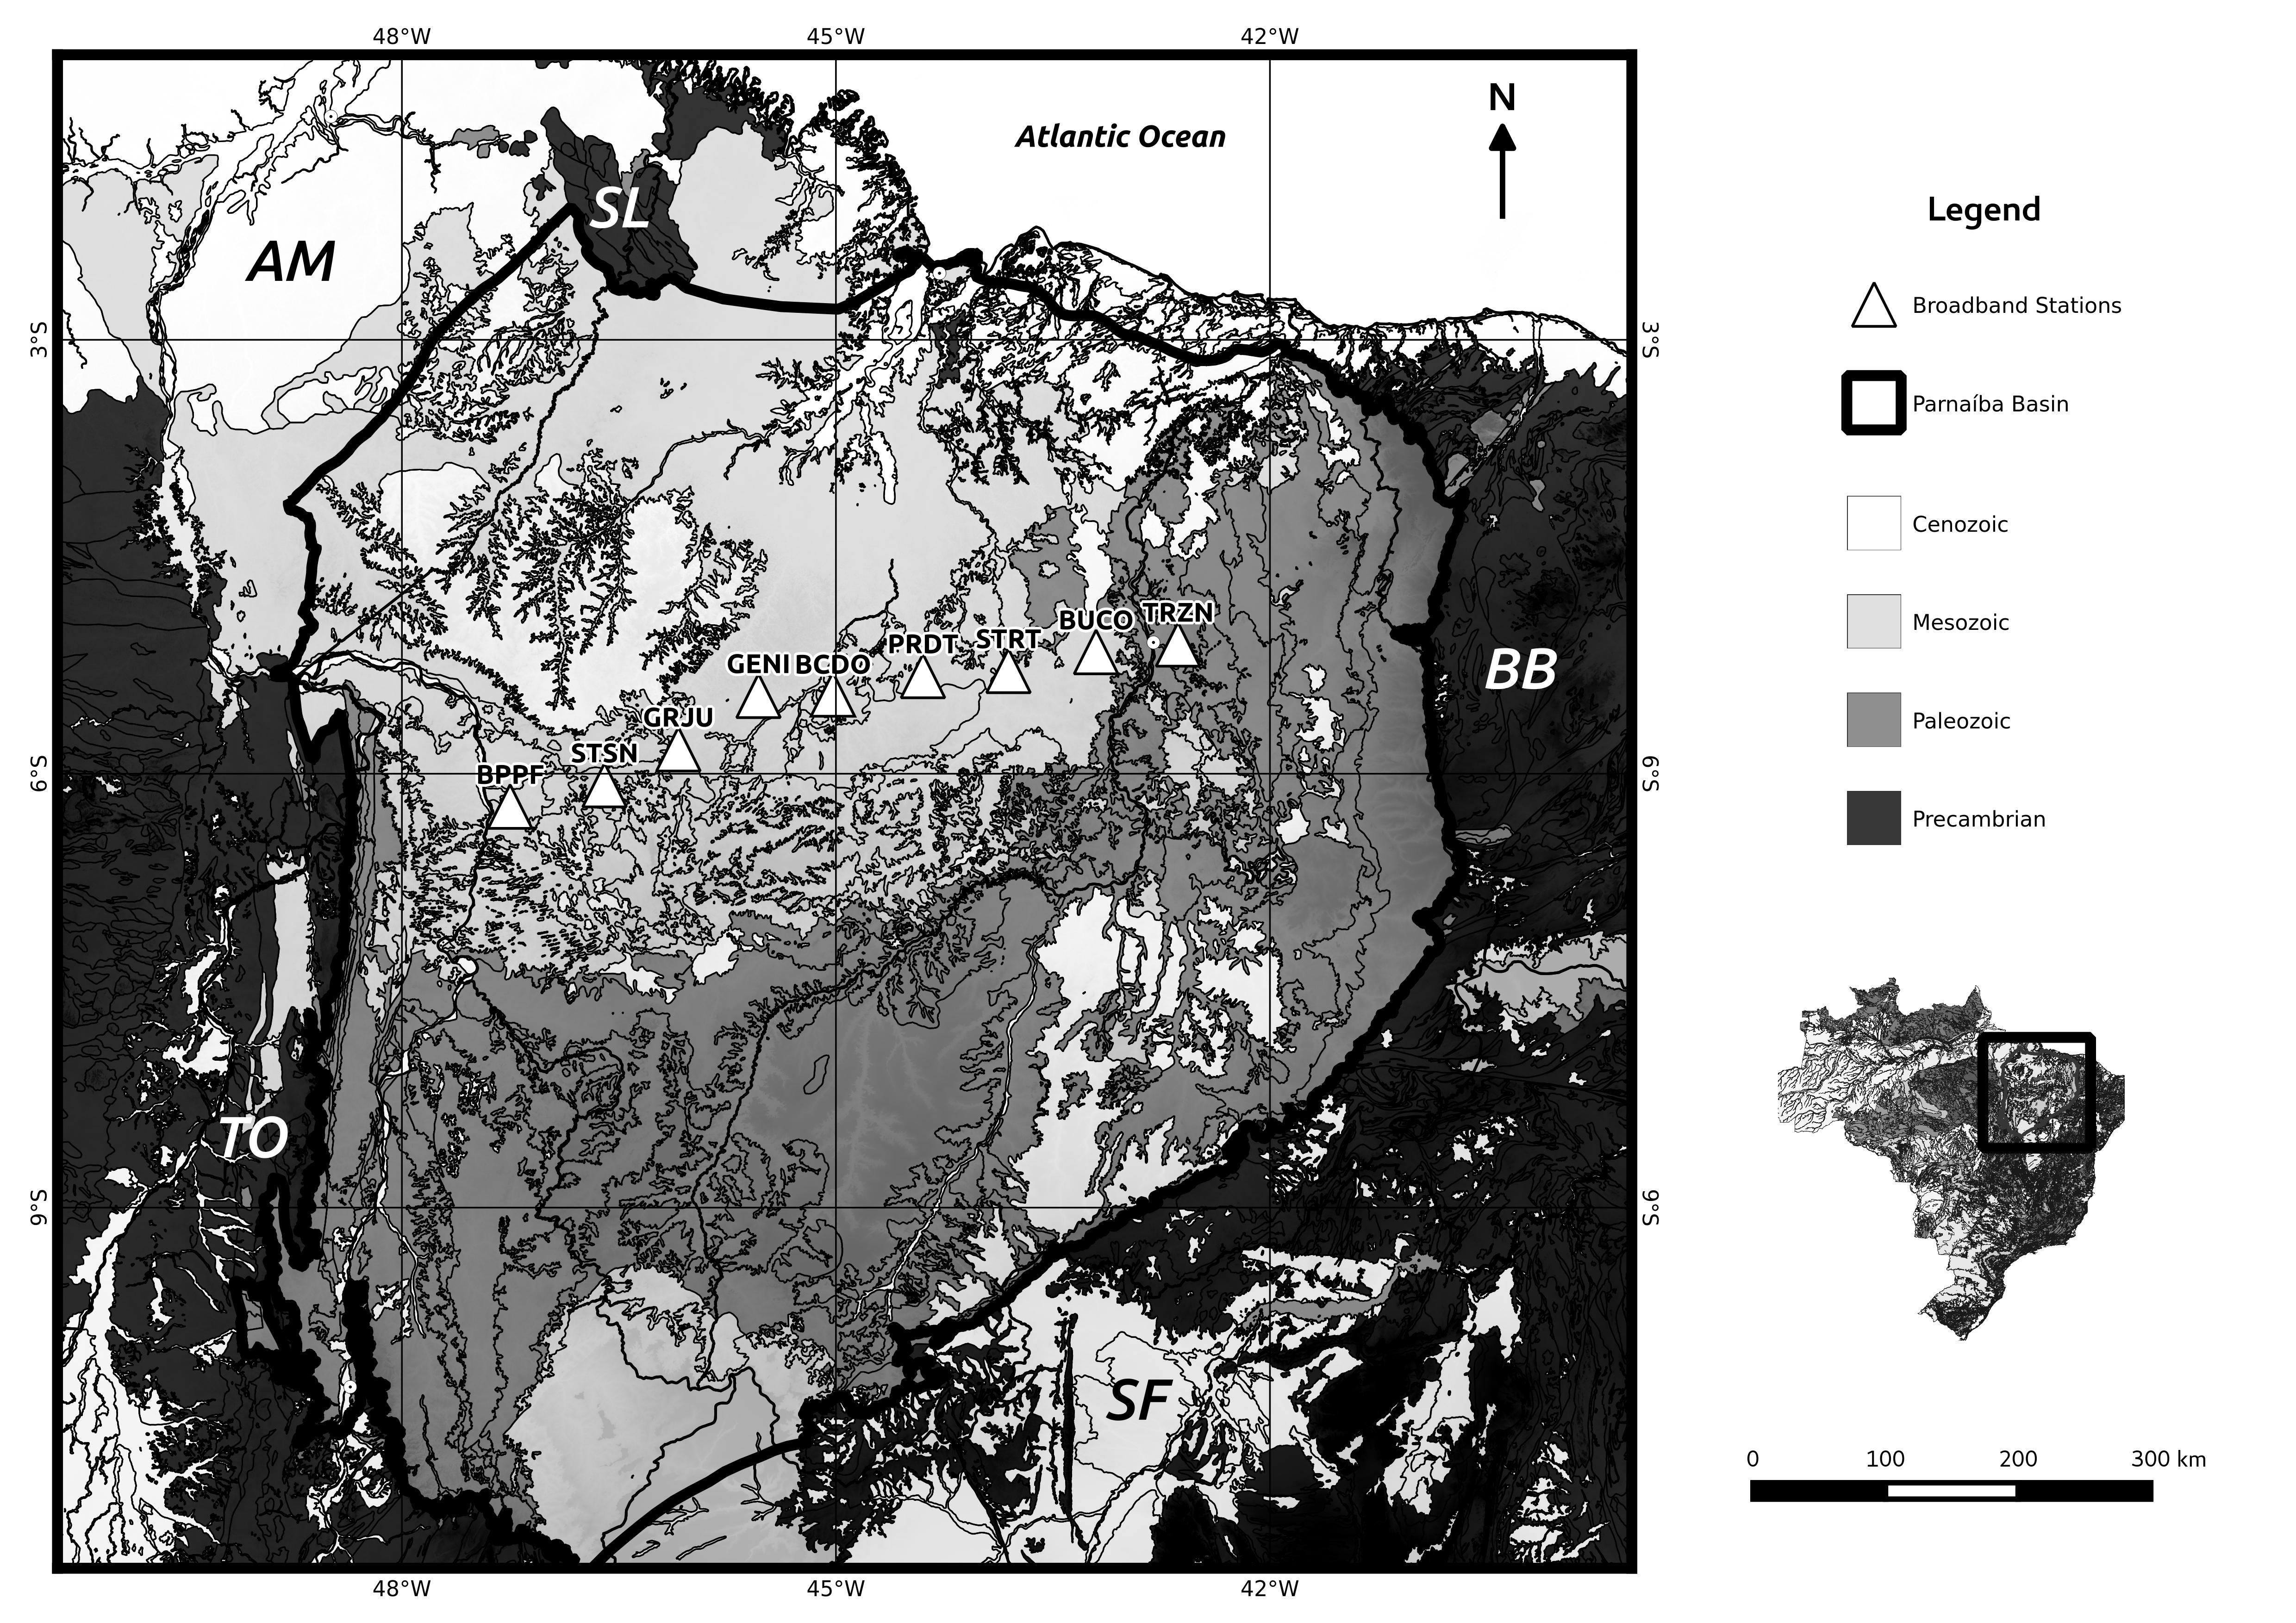
\includegraphics[width=\textwidth]{Fig/Mapa_geologico_BP_grey.pdf}
\caption{Geological Map with the location of PBAP project stations. AM, Amazonian Craton; BB, Borborema Province; SF, São Francisco Craton; SL, São Luís Craton; TO, Tocantins Province.}
\label{mapa_estacoes_geologico}
\end{center}
\end{figure}

\pagebreak

\begin{figure}[!ht]
\begin{center}
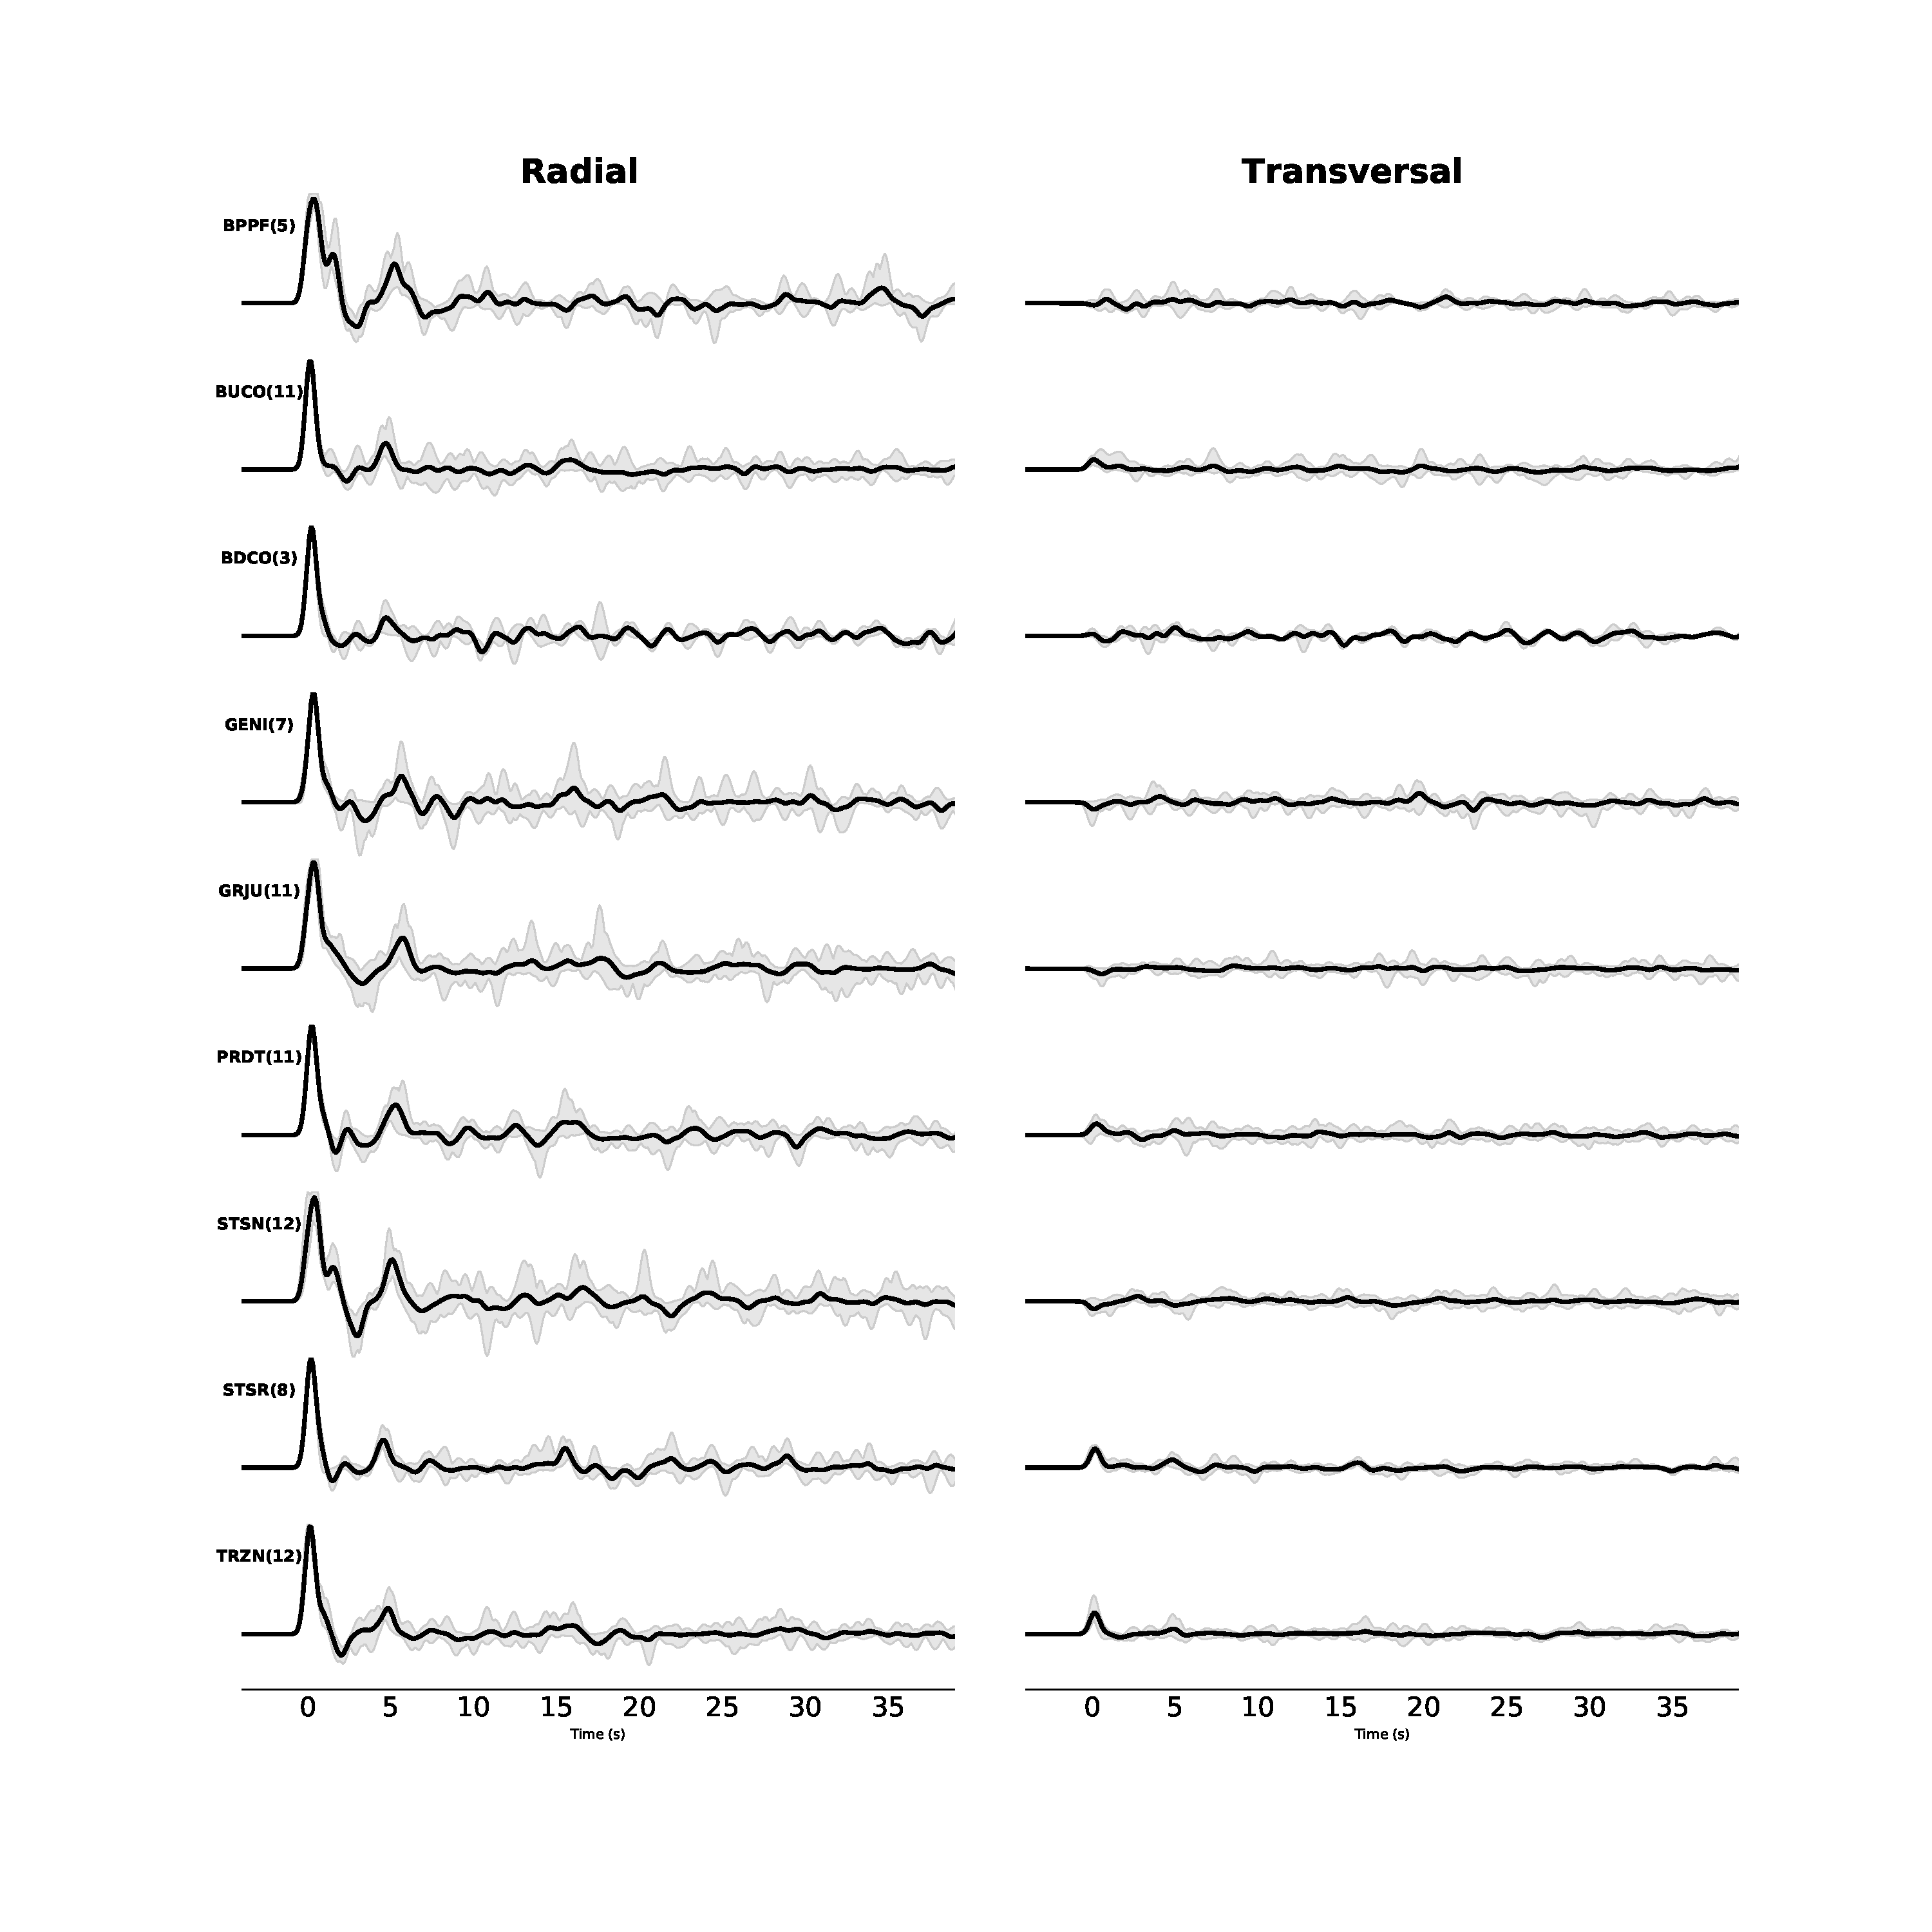
\includegraphics[width=\textwidth]{Fig/stations_FR.pdf}
\caption{Stacked receiver functions in the Parnaíba basin calculated with Gaussian filter width a = 2.5. Right and left panels show radial and transversal receiver functions, respectively, for each station. The number of waveforms stacked for each station are presented in round brackets. The maximum and minimum amplitude values of the receiver functions utilised are plotted in shaded gray.}
\label{estations_FR}
\end{center}
\end{figure}

\pagebreak

\begin{figure}[!ht]
\begin{center}
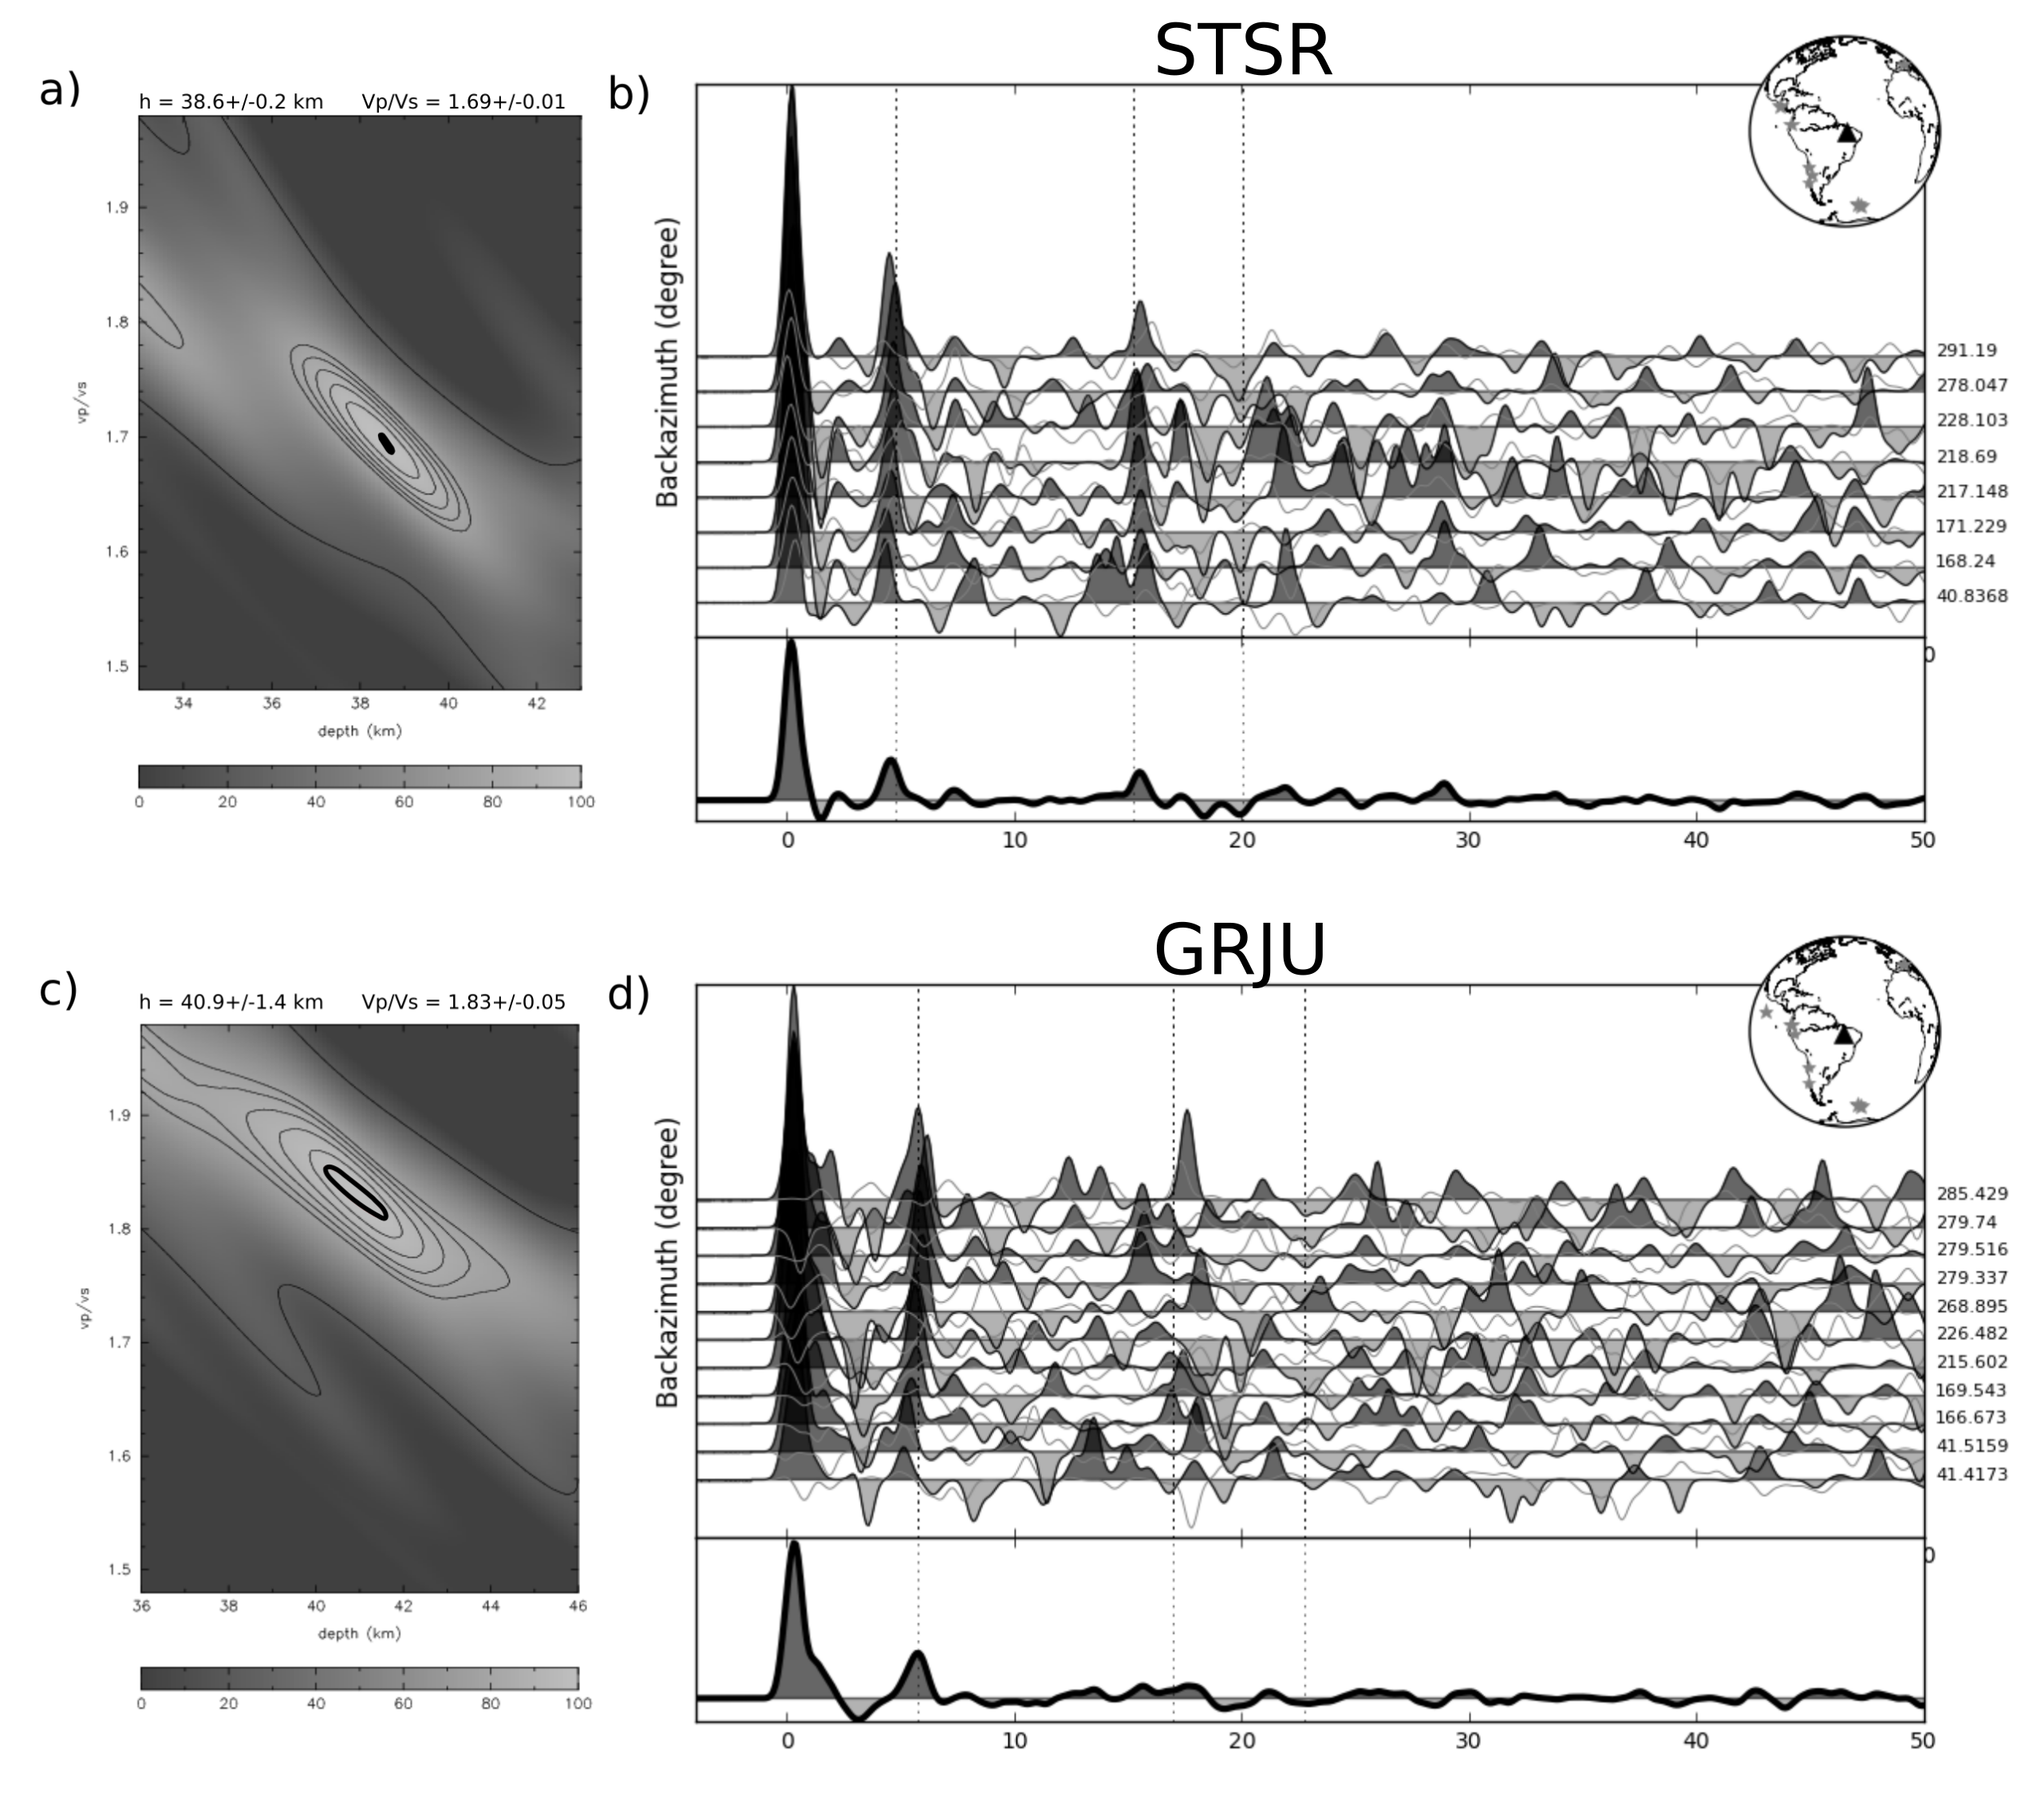
\includegraphics[width=\textwidth]{Fig/mosaico_GRJU_STSR.png}
\caption{Moisaic showing H-$\kappa$ stacking results for STSR (top) and GRJU (bottom) stations. a-c) display the receiver function stacked with the Ps, PpPs, and PpSs+PsPs phases times superimposed to the receiver functions and a figure showing the H-$\kappa$ stacking screen adopting a Vp of 6.3 $km/s$. b-d) display the receiver function, radial (black lines) and tranverse (red lines), sorted by backazimuth and at the right corner a map with the location of the earthquakes utilised (stars).}
\label{moisaic_FR}
\end{center}
\end{figure}

\pagebreak

\begin{figure}[!ht]
\begin{center}
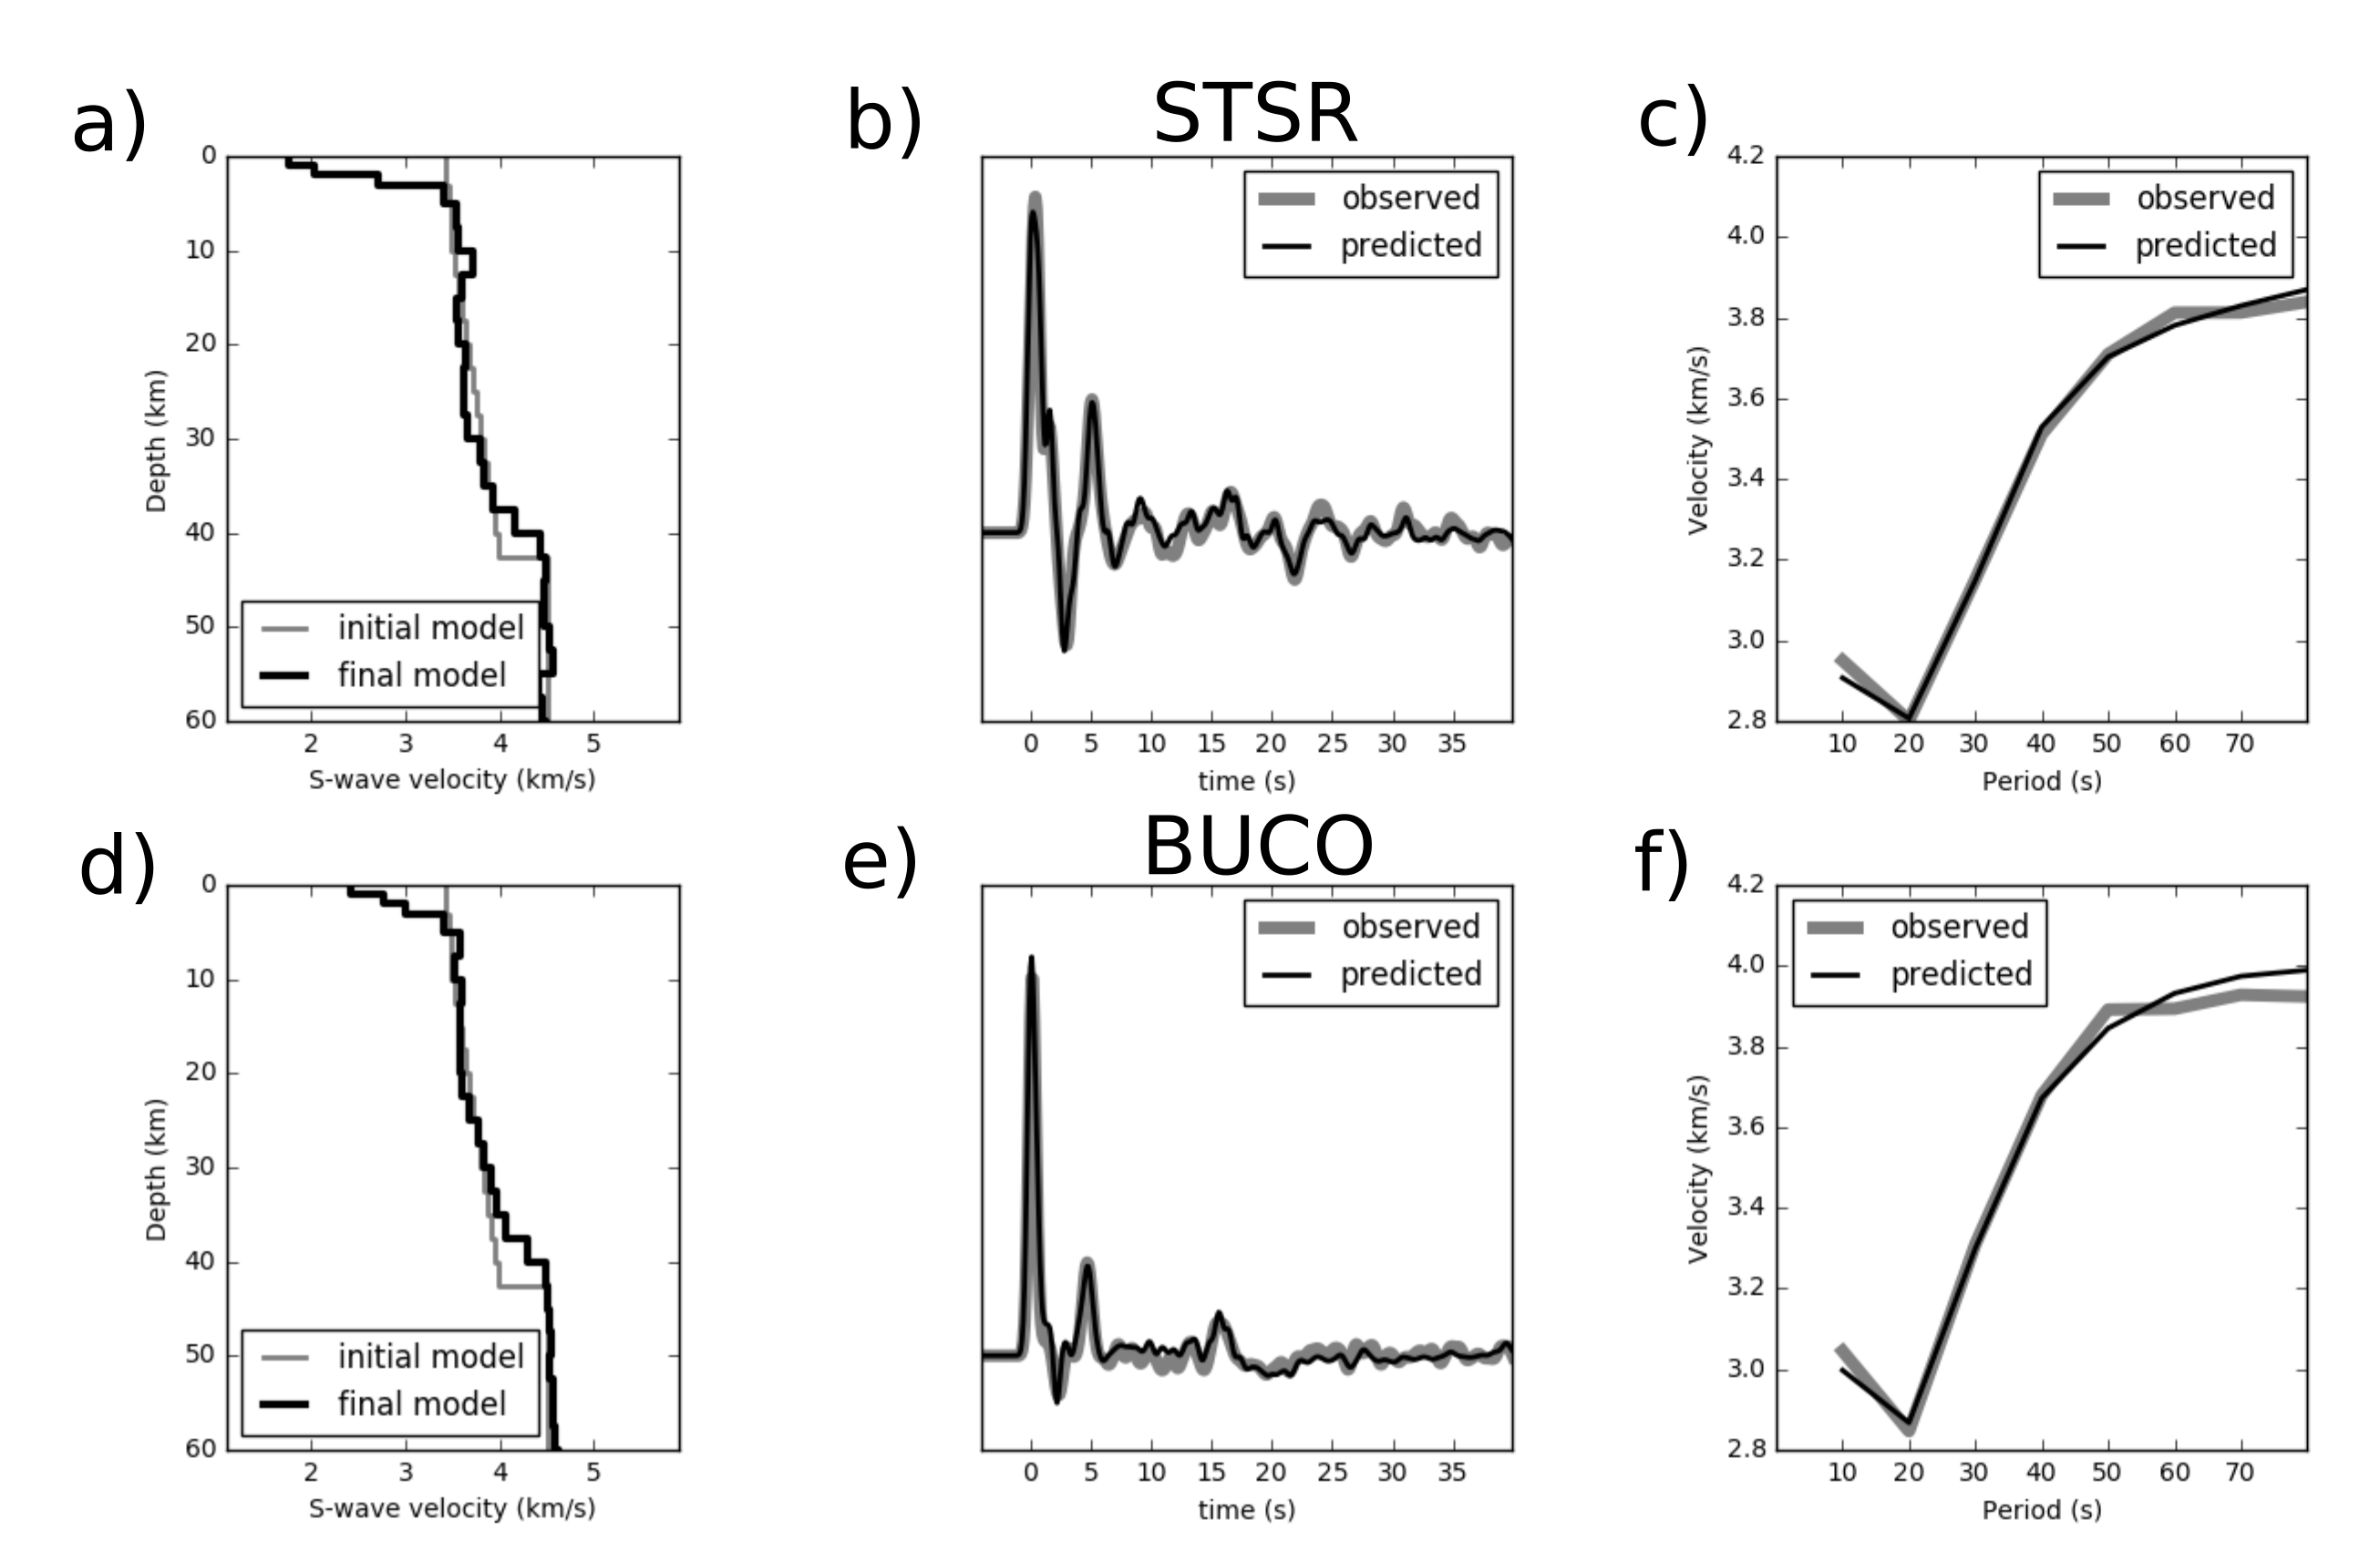
\includegraphics[width=\textwidth]{Fig/joint_inversion_results.png}
\caption{Joint inversion panels for STSN and BUCO stations. a-d) display the initial and final S-velocity models; b-e) fits between the receiver
functions observed and predicted; e-f) fits between the group velocities observed and predicted.}
\label{joint_inversion}
\end{center}
\end{figure}

\pagebreak
\begin{figure}[!ht]
\begin{center}
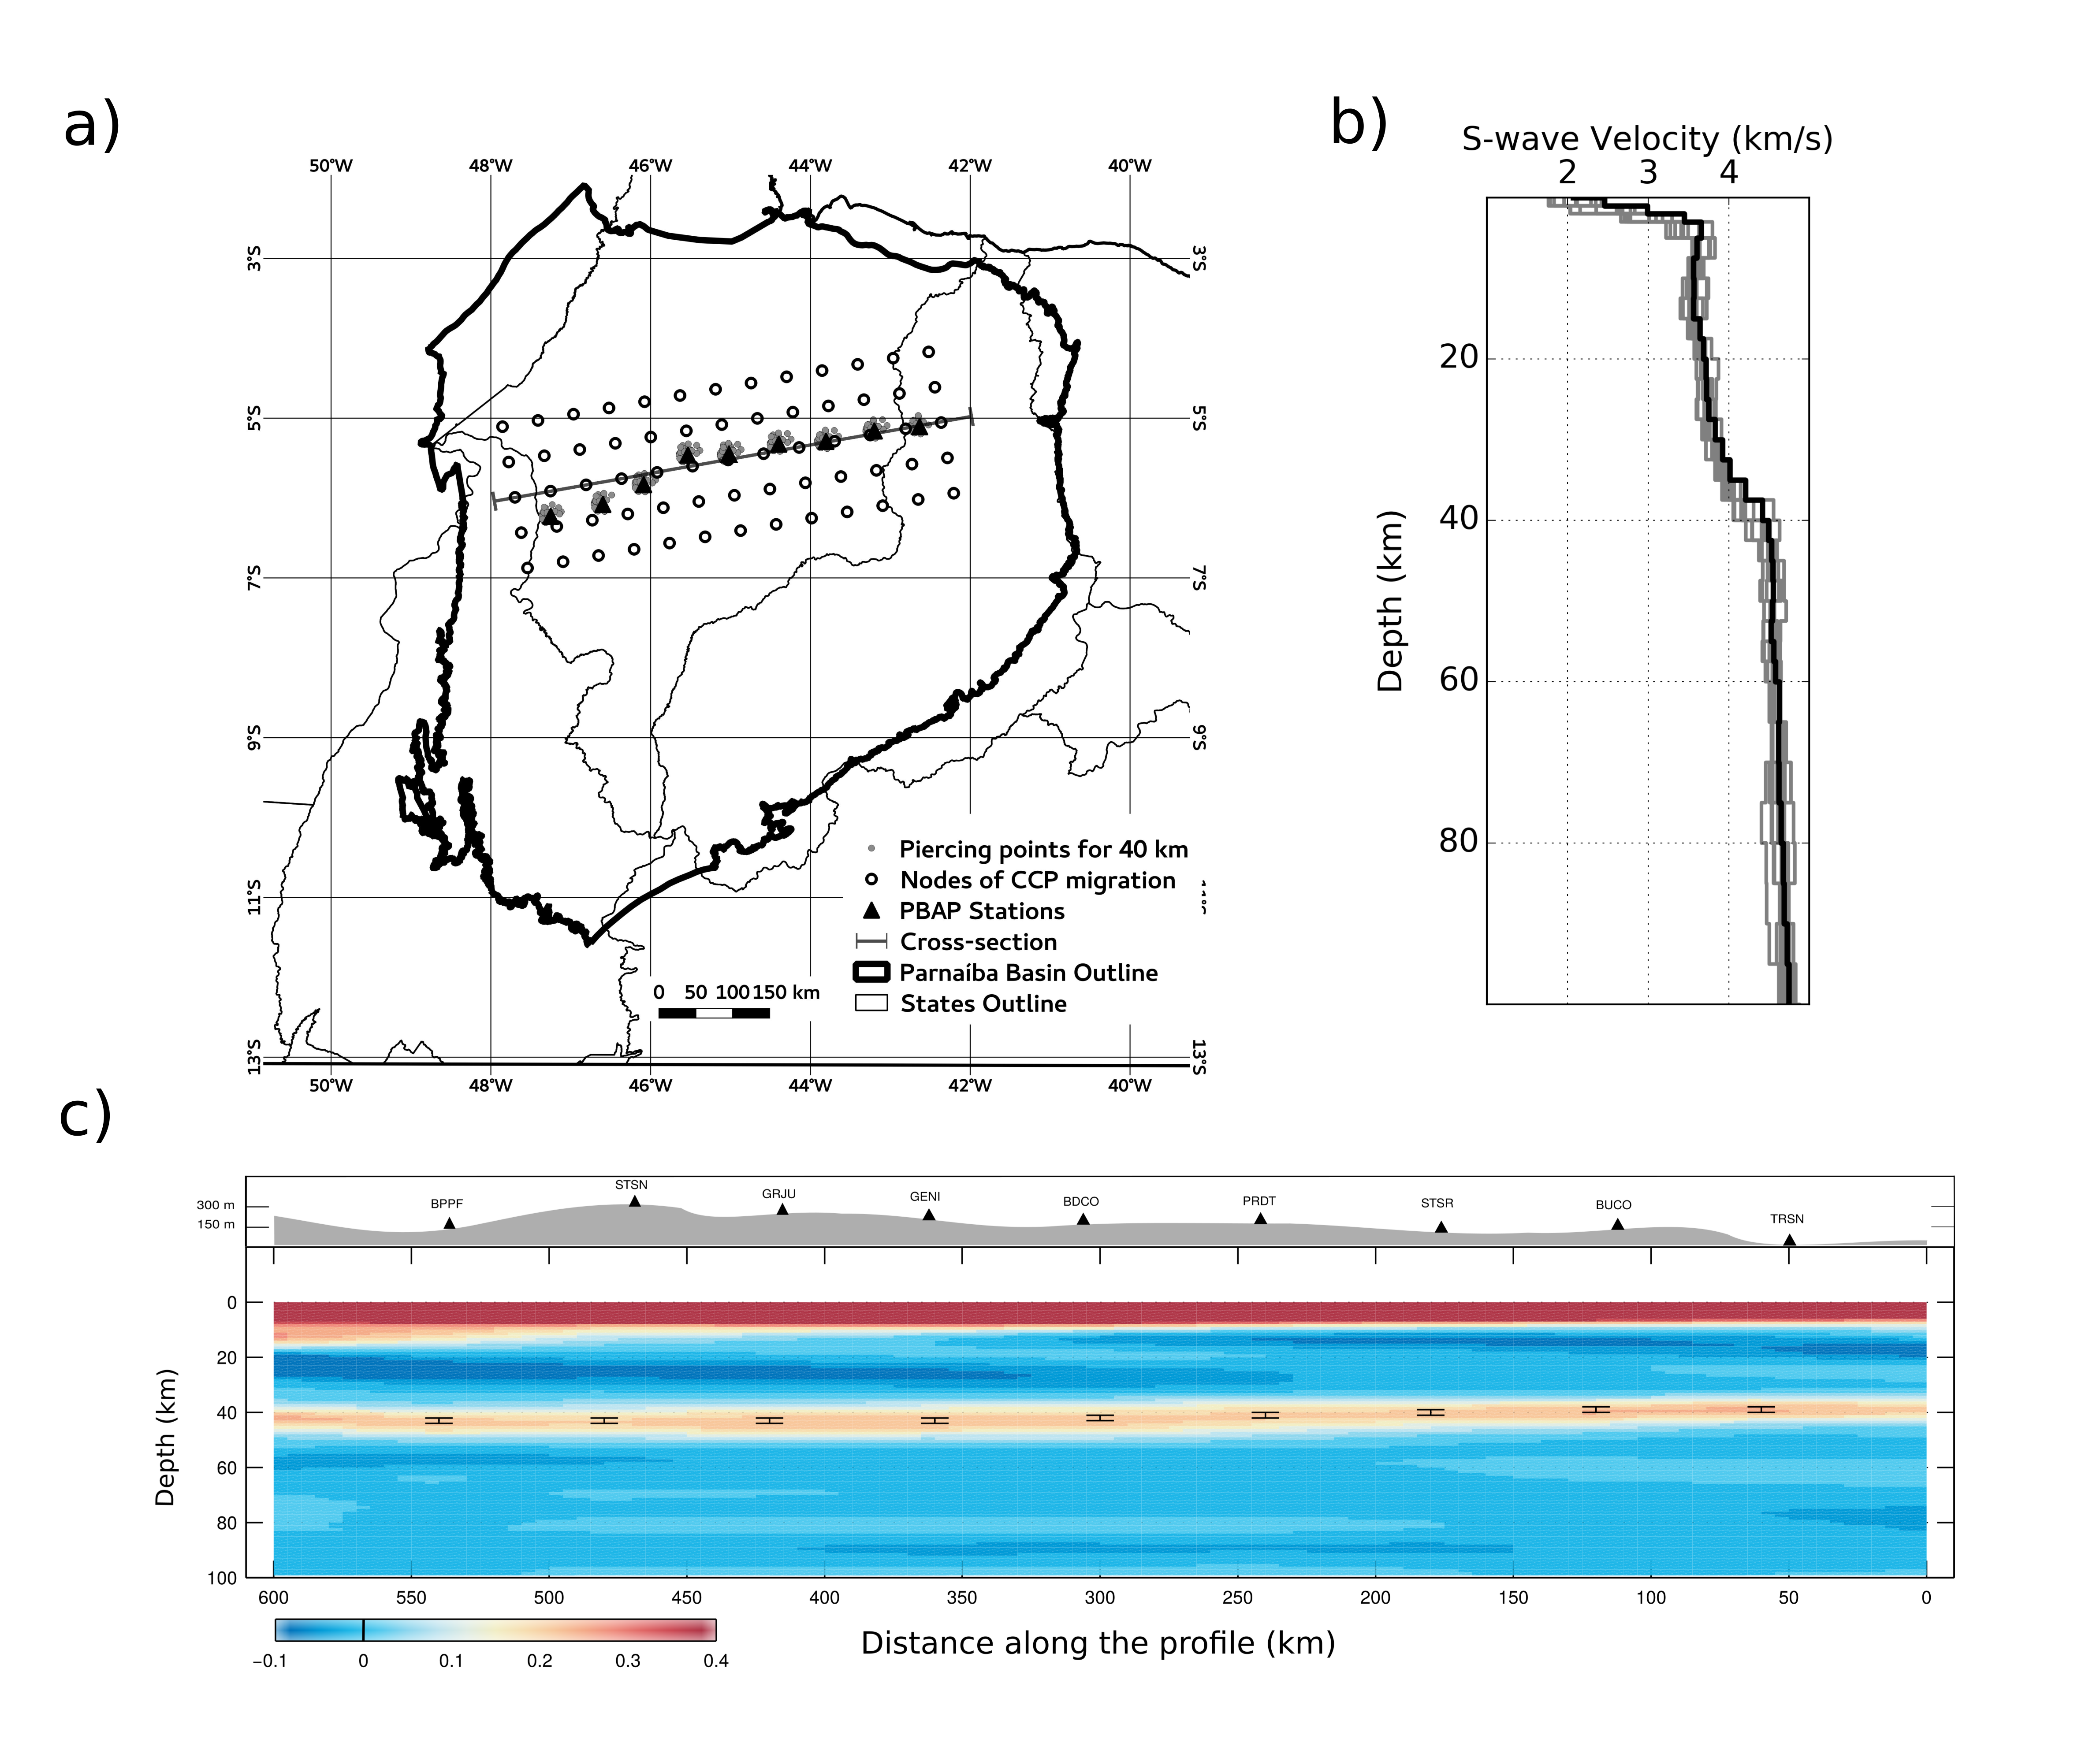
\includegraphics[width=\textwidth]{Fig/section_migration.png}
\caption{Mosaic with the piercing points map, S-wave velocity model and the migrated cross-section. a) map with the the seismic stations (black triangles), piercing points of the CCP migration (open circles) and CCP profile (black line). b) average S-wave velocity model for the PBAP stations. c) color-coded receiver function stacked amplitudes. Red colors indicate positive amplitudes (i.e., positive velocity contrast), while blue colors indicate negative amplitudes (i.e., negative velocity contrast). The black segments mark the location of the Moho Ps conversion at the crust–mantle boundary from bootstrapping.}
\label{moisaic_migration}
\end{center}
\end{figure}
 
\pagebreak

\begin{landscape}
\begin{figure}[!ht]
\begin{center}
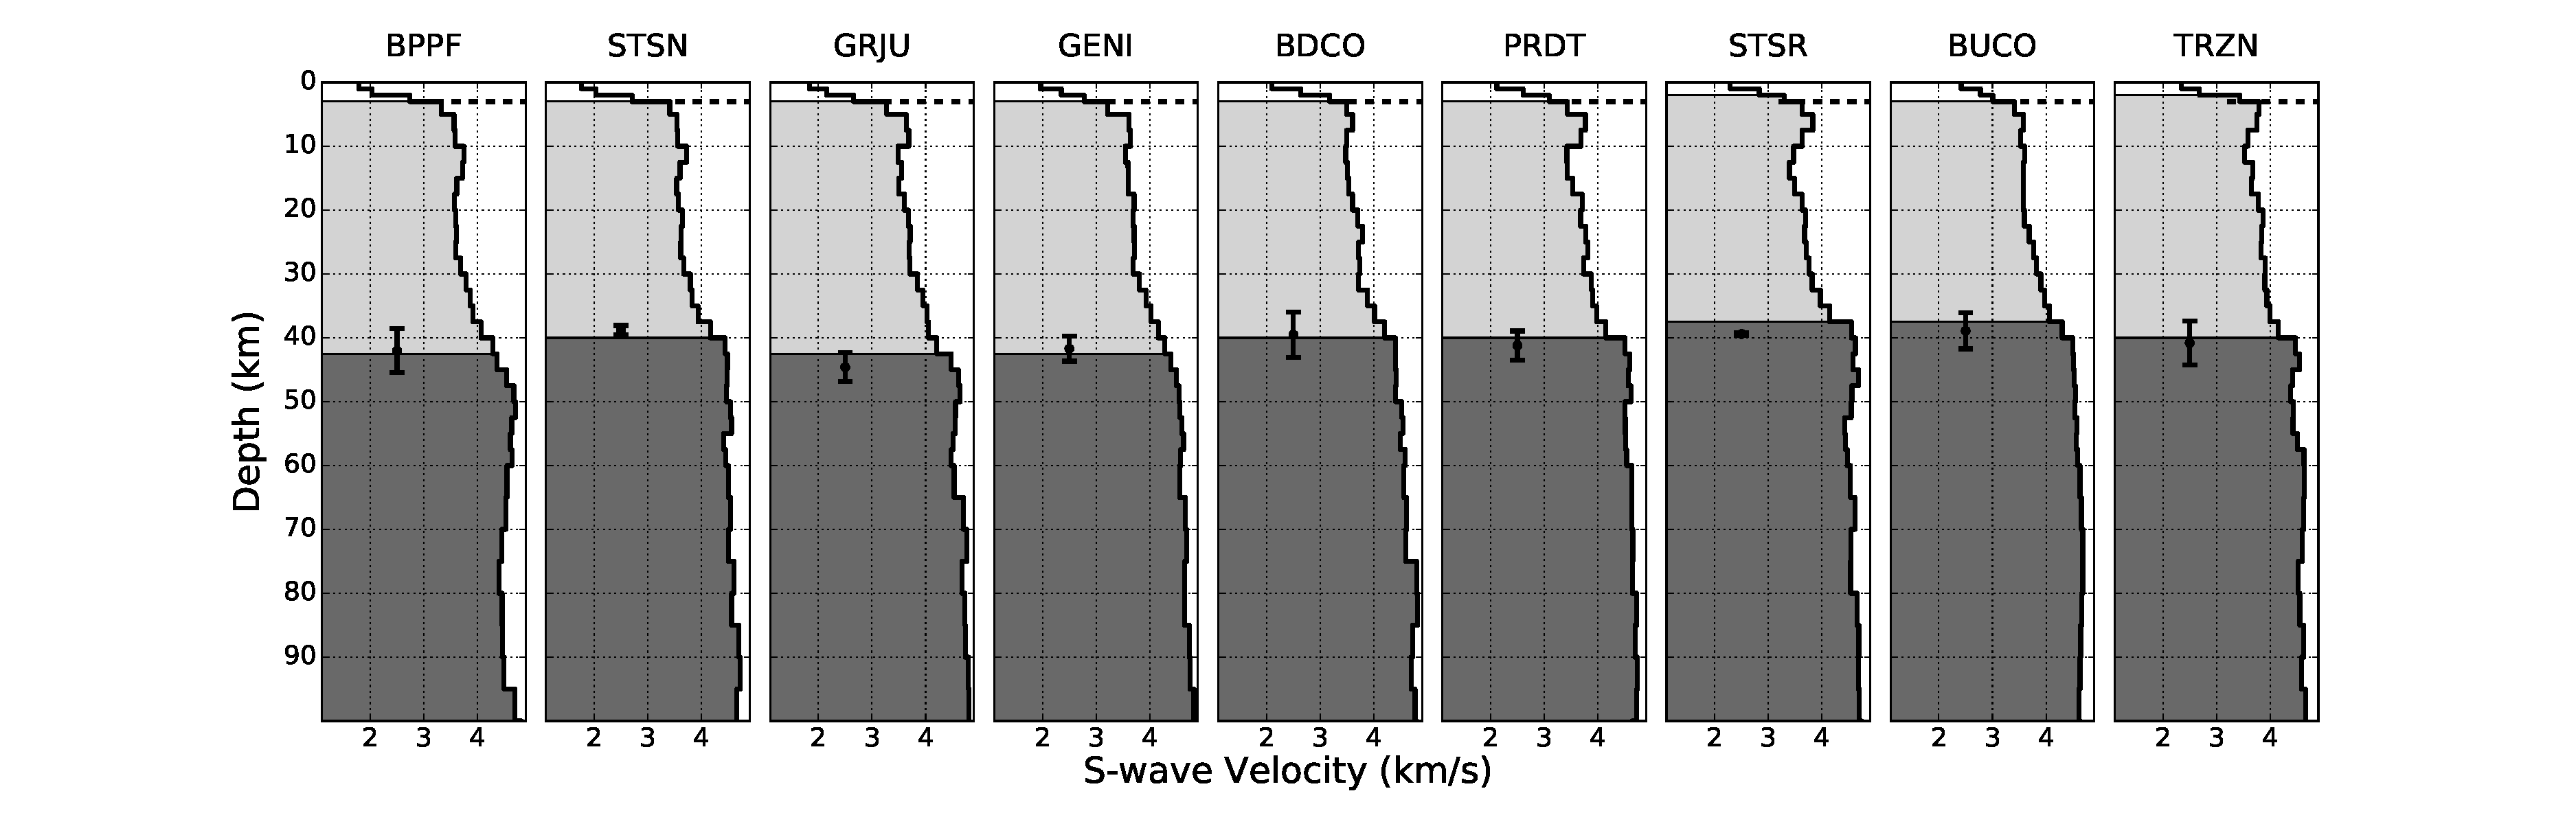
\includegraphics[width=1.6\textwidth]{Fig/section_joint_inversion_25.pdf}
\caption{Joint inversion models for each station sorted according the station location in Figure \ref{mapa_estacoes_geologico}. Colors represent S-wave velocities: The sedimentary layer, > 3.2 $km/s$ (white); crust, between 3.2 to 4.3 $km/s$ (gray); and mantle, < 4.3 $km/s$ (dark gray). These values are based in models calculated from \cite{mooney_crust_1998}. Dashed line represents the 3 km depth and the black segments are the H-$\kappa$ stacking results with error estimates, Adopting a Vp of 6.4 $km/s$.}
\label{moisaic_joint_inversion}
\end{center}
\end{figure}
\end{landscape}

\end{document}
